\chapter{Generalidades}
\label{cap:generalidades}

% ===================================================================
\section{Problemática}
\label{sec:problematica}
% ===================================================================
% NOTA DE ESTRUCTURA (06-10-2026)
% Reescrita a partir de la observación del jurado: el problema se enuncia en
% la primera página; después se delimita el dominio, se dimensiona y se
% justifica, y recién entonces se analizan las causas y los efectos (sección
% del árbol) y la brecha de investigación. Cada figura y cada tabla se
% introduce y se explica en función del problema. El diagnóstico completo y
% el plan de los pasos siguientes están en REESTRUCTURACION.md, en esta misma
% carpeta.
%
% Regla que se mantiene: la problemática es narrativa y carga el peso de las
% citas; el árbol es la síntesis causal y remite a la evidencia de aquí.
% ===================================================================

\subsection{Definición del problema}
\label{sec:problema}

Los primates de la Amazonía son difíciles de seguir. Viven en un bosque de
vegetación densa, y muchas de sus especies son crípticas o poco abundantes, de
modo que los encuentros directos son escasos: son las condiciones que hacen del
bosque tropical uno de los ambientes más difíciles para el monitoreo de fauna
\citep{zwerts_methods_2021}. El monitoreo acústico pasivo (PAM, por sus siglas en
inglés) sortea esa dificultad: grabadoras autónomas instaladas en el bosque
registran el sonido de forma continua durante semanas o meses, sin intervenir en
el ecosistema \citep{gibb_2018}.

Esta tesis trabaja con el material de un programa de ese tipo. En el Tambopata
Research Center, en la Reserva Nacional Tambopata (Madre de Dios), el 8 Primates
Project, una iniciativa de ciencia ciudadana de Rainforest Expeditions que dirige
Mark Bowler, estudia las ocho especies de primates del río Tambopata
\citep{wiredamazon_8primates}: el tamarino de Weddell (\textit{Leontocebus
    weddelli}), el tití de Toppin (\textit{Plecturocebus toppini}), el capuchino de
cabeza chata (\textit{Cebus cuscinus}), el mono araña peruano (\textit{Ateles
    chamek}), el mono nocturno (\textit{Aotus azarae}), el capuchino de cabeza
grande (\textit{Sapajus macrocephalus}), el mono aullador rojo boliviano
(\textit{Alouatta sara}) y el mono ardilla boliviano (\textit{Saimiri
    boliviensis}), ocho de las 42 especies de primates que se registran en el Perú
\citep{pacheco_lista_2021}. Con grabadoras desplegadas en el bosque, el proyecto
reúne bibliotecas de llamadas de cada especie y las usa para detectar a los monos
y para establecer un programa de monitoreo con pobladores locales
\citep{wiredamazon_8primates}. En adelante, \emph{equipo de investigación}
designa al de ese proyecto.

Para que las grabaciones sirvan a ese fin, cada vocalización tiene que
encontrarse dentro del audio, delimitarse en el tiempo y en la frecuencia, y
recibir la especie y el tipo de llamada. Esa tarea, la \emph{anotación}, la hace a
mano un especialista que conoce el repertorio de cada especie, y es el paso más
lento de todo el proceso. El problema que aborda esta tesis se enuncia así:

\begin{quote}
    Anotar las vocalizaciones de primates neotropicales en grabaciones de
    monitoreo acústico pasivo exige más tiempo de especialista del que está
    disponible.
\end{quote}

\subsection{El material y su anotación}
\label{sec:dominio}

El material de partida se produce en dos pasos. Primero, grabadoras AudioMoth,
dispositivos de bajo costo y de código abierto \citep{hill_audiomoth_2018},
registran el sonido del bosque en archivos WAV a 44,1\,kHz. Después, un
especialista abre cada grabación en Raven Pro, el programa de análisis de sonido
del Laboratorio de Ornitología de Cornell con que trabaja el equipo
\citep{raven_pro}, e inspecciona su espectrograma: la imagen
que muestra la energía del sonido según el tiempo, en el eje horizontal, y la
frecuencia, en el vertical. Sobre esa imagen dibuja un rectángulo alrededor de
cada vocalización y le asigna dos etiquetas, la especie y el tipo de llamada,
escritas como códigos: dos letras para la especie, que la
Tabla~\ref{tab:resumen-dataset} asocia a su nombre, y dos o tres para el tipo de
llamada. La Figura~\ref{fig:annotation-example} muestra una de esas anotaciones: una sílaba
de contacto del tamarino de Weddell (\texttt{LW/CS}), delimitada por sus
instantes de inicio y fin ($t_{\text{ini}}$ y $t_{\text{fin}}$) y por su
frecuencia mínima y máxima ($f_{\min}$ y $f_{\max}$).

\begin{figure}[htbp]
    \centering
    \caption{Anotación tiempo--frecuencia en Raven}
    \label{fig:annotation-example}
    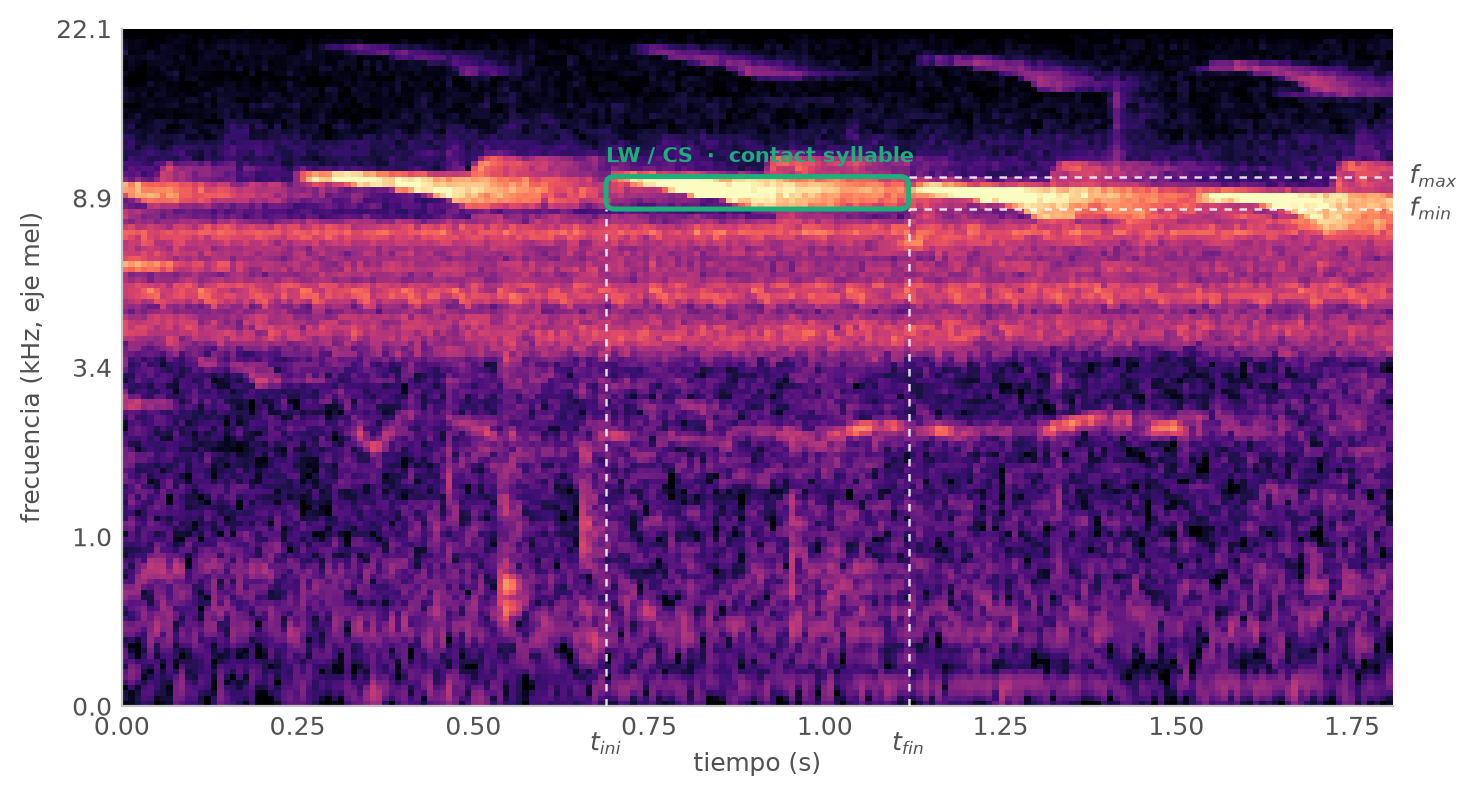
\includegraphics[width=0.78\textwidth]{capitulos/01_generalidades/figures/annotation_example.png}
\end{figure}

Esa caja con sus dos etiquetas es la unidad de información que produce el
análisis; el documento llama \emph{anotación} tanto a la tarea como a su
producto. Sus cuatro coordenadas
resumen la duración, el ancho de banda y la frecuencia central de la
vocalización, información que el analista usa directamente
\citep{escobar-amado_computer_2024}. El tipo de llamada, por su parte, conecta la
anotación con el comportamiento: el repertorio de estas especies incluye llamadas
de contacto, alarmas aéreas y terrestres, duetos, llamadas de alimento y
vocalizaciones agresivas, de modo que saber qué tipo
de llamada se emitió informa más que saber que la especie estuvo presente.

La Tabla~\ref{tab:resumen-dataset} resume, por especie, el material que el equipo
entregó para esta tesis: cuántas grabaciones hay y cuántas horas suman, cuántas de
ellas tienen anotaciones, cuántos minutos ocupan las vocalizaciones anotadas y qué
fracción del tiempo grabado representan.

\begin{table}[htbp]
    \centering
    \caption{Material recibido por especie}
    \label{tab:resumen-dataset}
    \small
    % Códigos verificados contra src/data/species.py y contra el repertorio del
    % marco conceptual. No cambiar sin actualizar también aquella y el
    % vocabulario del capítulo 4. Las filas las escribe el cuaderno.
    \begin{tabular}{@{}L{6.1cm}rrrrr@{}}
        \toprule
                                  & \multicolumn{2}{c}{\textbf{Grabado}} & \multicolumn{3}{c}{\textbf{Anotado}}                      \\
        \cmidrule(lr){2-3}\cmidrule(lr){4-6}
        \textbf{Especie (código)} & \thead{N.\textsuperscript{o}}        & \thead{Horas} & \thead{N.\textsuperscript{o}}
                                  & \thead{Evento\\(min)}               & \thead{Fracción\\(\char37)}                               \\
        \midrule
                Mono aullador (AS) & 808 & 7,57 & 778 & 324,6 & 71,5 \\
        Capuchino de cabeza grande (SM) & 659 & 6,13 & 582 & 16,6 & 4,5 \\
        Mono araña peruano (AC) & 561 & 6,07 & 384 & 30,7 & 8,4 \\
        Tamarino de Weddell (LW) & 530 & 5,28 & 410 & 47,5 & 15,0 \\
        Tití de Toppin (PT) & 375 & 3,35 & 320 & 94,3 & 47,0 \\
        Mono ardilla boliviano (SB) & 290 & 3,08 & 256 & 12,2 & 6,6 \\
        Mono nocturno (AA) & 117 & 1,10 & 82 & 2,5 & 3,8 \\
        Capuchino de cabeza chata (CC) & 16 & 0,11 & 7 & 0,1 & 1,2 \\
        \midrule
        \textbf{Total} & \textbf{3\,356} & \textbf{32,69} & \textbf{2\,819} & \textbf{528,5} & \textbf{26,9} \\
        \bottomrule
    \end{tabular}
\end{table}

En total son \gRecordings{} grabaciones y \gHours{} horas, de las cuales
\gAnnotated{} grabaciones (\gAnnotatedHours{} horas) tienen anotaciones, y las
vocalizaciones anotadas ocupan \gEventMinutes{} minutos, el \gEventShare{}\,\% de
lo grabado. Dos rasgos de la tabla importan para el problema. El primero es qué
representa: no es todo lo que el proyecto grabó, sino la selección que el equipo
organizó por especie para anotarla, con un criterio que el material no
documenta, y por eso la mayor parte está anotada. Su tamaño lo confirma:
\gHours{} horas equivalen a menos de un día y medio de registro continuo de una
sola grabadora, de modo que incluso este material, el único anotado de que se
dispone para estas especies, es una muestra mínima de lo que el PAM puede
producir. El segundo es el desequilibrio entre
especies: la fracción del tiempo grabado que ocupan las vocalizaciones anotadas
varía en más de un orden de magnitud, desde el mono aullador, cuyos aullidos son
largos y continuos, hasta el capuchino de cabeza chata, del que apenas hay
material. Ese desequilibrio, que responde tanto a la duración de las llamadas de
cada especie como a lo que se llegó a grabar y a anotar, condiciona la
construcción del conjunto de datos y la manera de evaluar un detector.

\subsection{Magnitud del problema}
\label{sec:magnitud}

El problema existe porque grabar se volvió barato y analizar no. Del lado de la
recolección, una grabadora AudioMoth tiene un costo de fabricación de unos
43 dólares estadounidenses \citep{hill_audiomoth_2018}, y los sensores de bajo
costo y de código abierto permiten desplegar redes de muchos micrófonos a escala
\citep{gibb_2018}; el costo de grabar y de almacenar cayó lo suficiente como para
hacer viable la captura continua \citep{stowell_computational_2022}. La
consecuencia se mide en horas. Una sola grabadora en registro continuo produce
24 horas de audio por día, unos 7,6\,GB en el formato del material de esta tesis
(44,1\,kHz, 16 bits, un canal), y una red modesta de diez grabadoras acumula
7\,200 horas en un mes. Los proyectos reales operan a esa escala: el detector de
aullidos de lobo HOWLish se construyó sobre 50\,137 horas de paisaje sonoro, en
las que se anotaron a mano 841 eventos de aullido
\citep{Campos_Krofel_Rio-Maior_Renna_2025}. Y el uso del método crece: una
revisión sistemática del PAM terrestre registró un aumento de más de quince veces
en el número de publicaciones entre 1992 y 2018 \citep{sugai_terrestrial_2019}.

Del lado del análisis, la revisión sigue siendo mayoritariamente manual. El
análisis bioacústico de vocalizaciones se realiza sobre todo mediante la
inspección manual de las grabaciones, un proceso muy subjetivo y que consume
mucho tiempo \citep{romero-mujalli_utilizing_2021}, y más de la mitad de los
estudios de PAM terrestre revisados por \citet{sugai_terrestrial_2019} analizó el
audio a mano. \citet{romero-mujalli_utilizing_2021} lo resumen al señalar que hoy
el factor que limita la investigación con vocalizaciones animales es el análisis
de las grabaciones, y no la técnica para obtenerlas.

El costo de esa revisión se hace visible cuando se mide lo que ahorra asistirla.
Con detección automática, el análisis de un año de grabaciones del mono aullador
negro y dorado requirió un tiempo equivalente al 2\,\% de la duración grabada
\citep{perez-granados_passive_2021}. En los casos que comparan directamente con
la revisión manual, depurar los falsos positivos de un sistema semiautomático
para cuatro especies de primates costó entre el 3 y el 5\,\% del tiempo del
procesamiento humano \citep{heinicke_2015}, HOWLish redujo 15 veces el tiempo del
operador \citep{Campos_Krofel_Rio-Maior_Renna_2025} y un detector de llamadas de
langur redujo en un 87\,\% la carga de revisión manual \citep{hong_deep_2026}.
Leídas a la inversa, esas cifras indican que la revisión sin asistencia costaba,
según el caso, entre unas ocho y unas treinta veces más tiempo. Y todas
corresponden a detectar una o pocas especies: la anotación que requiere el
dominio de esta tesis, con caja y tipo de llamada para varias especies, exige más
decisiones por evento, y recolectar etiquetas que delimitan cada evento ya es, de
por sí, lo que más tiempo consume en la detección de eventos sonoros
\citep{koga_lead_2024}.

El tercer factor es quién puede hacer ese trabajo. Asignar el tipo de llamada
exige conocer el repertorio de cada especie, y el tiempo de analistas con esa
formación es escaso: la falta de tiempo-persona de analistas entrenados es el
cuello de botella habitual de la bioacústica \citep{stowell_computational_2022},
y recolectar anotaciones es el principal obstáculo para construir métodos
automáticos \citep{nguyen_assessing_2021}. La respuesta habitual es repartir la
anotación entre varias personas \citep{koga_lead_2024}, lo que alivia el volumen
a costa de introducir criterios distintos en un mismo conjunto de datos, un efecto
que reaparece entre las causas del problema.

\subsection{Relevancia}
\label{sec:relevancia}

Reducir el tiempo de anotación importa, en primer lugar, por lo que está en juego
para las especies. Los primates son un componente esencial de la biodiversidad
tropical; alrededor del 60\,\% de sus especies está amenazado de extinción y el
75\,\% tiene poblaciones en declive \citep{estrada_impending_2017}. Entre las ocho
especies de esta tesis, el mono araña peruano figura como En Peligro en la Lista
Roja de la Unión Internacional para la Conservación de la Naturaleza: se estima que su población se redujo al menos a la mitad en los
últimos 45 años por la caza y la pérdida de hábitat, y la ganadería y la
deforestación están extendidas en el sureste del Perú \citep{alves_ateles_2021}.
Conservar poblaciones así exige seguirlas en el tiempo, y ese seguimiento es la
base de las decisiones de conservación, con la dificultad añadida que imponen los
bosques tropicales \citep{zwerts_methods_2021}.

En segundo lugar, el PAM es una herramienta adecuada para ese seguimiento. Los
sensores acústicos no son invasivos, suelen ser omnidireccionales y ofrecen un
área de detección mayor y menos restricciones taxonómicas que las cámaras
trampa; permiten muestrear durante periodos largos con poco esfuerzo manual, lo
que aumenta la probabilidad de detectar especies raras o poco vocales
\citep{gibb_2018}. En primates, la detección automática sobre grabaciones de PAM
ya se ha usado para estimar la ocupación de varias especies en un bosque de Costa
de Marfil \citep{kalan_towards_2015} y para describir los patrones de
vocalización de monos aulladores en Brasil
\citep{perez-granados_passive_2021,do_nascimento_passive_2021}. Aun así, el PAM
rara vez se ha aplicado al monitoreo de primates
\citep{perez-granados_passive_2021}, y sus ventajas solo se materializan si el
análisis acompaña a la recolección: los programas de monitoreo deben ser
estandarizables, escalables y financieramente sostenibles \citep{gibb_2018},
condiciones que un análisis enteramente manual no cumple a la escala que el PAM
hace posible.

En tercer lugar, el problema es relevante para la informática. Convertir una
grabación en anotaciones con la forma que usa el especialista exige resolver en un
solo sistema la localización de cada vocalización en tiempo y en frecuencia y su
clasificación fina por especie y tipo de llamada, es decir, llevar la detección de
objetos de la visión por computadora a una señal que no es una imagen natural. Y
lo es para el
equipo de investigación, que es quien sostiene el monitoreo: cada hora de
especialista que se ahorra en la anotación queda disponible para la
interpretación ecológica de los datos.

% ===================================================================
\section{Árbol de problemas}
\label{sec:arbol}
% ===================================================================

El árbol de problemas ordena en relaciones de causa y efecto la evidencia de la
sección anterior. Se construye con el heurístico de \citet{vesely_problem_2008}:
el problema central ocupa el centro, sus causas se ubican debajo y sus efectos
encima, y cada flecha se lee como ``conduce a''. El árbol no cuantifica esas
relaciones; su función es explicar por qué ocurre el problema y qué provoca, y
servir de puente hacia los objetivos, que se derivan de él invirtiendo su
lógica. La
Figura~\ref{fig:problem-tree} lo resume, y las subsecciones que siguen
desarrollan cada elemento.

\begin{figure}[htbp]
    \centering
    \caption{Árbol de problemas}
    \label{fig:problem-tree}
    \resizebox{\textwidth}{!}{%
        \begin{tikzpicture}[
                % Las cajas llevan el enunciado abreviado del apartado que las
                % desarrolla. El font va después de `caja`, que impone \small y
                % descuadraba las alturas.
                % Sin partición de palabras: en cajas de 44 mm cortaba "espe-cies".
                nodo/.style={caja, font=\footnotesize, align=center, text width=44mm,
                        minimum height=15mm, inner sep=4pt,
                        execute at begin node={\hyphenpenalty=10000\exhyphenpenalty=10000}},
                efecto/.style={nodo, draw=ambar!80!black, fill=ambar!8},
                causa/.style={nodo, draw=azul!70, fill=azul!8, align=flush left,
                        minimum height=37mm},
                central/.style={nodo, draw=azul!80!black, fill=azul, text=white,
                        text width=124mm, minimum height=17mm},
                sube/.style={-{Stealth[length=2.2mm]}, thick, draw=ambar!80!black},
                nace/.style={-{Stealth[length=2.2mm]}, thick, draw=azul!70},
                liga/.style={-{Stealth[length=2.2mm]}, thick, dashed, draw=azul!70},
                franja/.style={font=\scriptsize\bfseries, rotate=90},
            ]
            % --- efectos ---
            \node[efecto] (e3) at (0, 10.3)
            {\textbf{E3.} La conservación decide con información tardía o
                incompleta};
            \node[efecto] (e1) at (-2.6, 7.7)
            {\textbf{E1.} El audio recolectado se acumula sin analizar};
            \node[efecto] (e2) at (2.6, 7.7)
            {\textbf{E2.} El análisis se limita a pocas especies y a sus
                llamadas más evidentes};
            % --- problema central ---
            \node[central] (pc) at (0, 5.1)
            {\textbf{PROBLEMA CENTRAL}\\[2pt] Anotar las vocalizaciones de primates
                neotropicales en grabaciones de monitoreo acústico pasivo exige más
                tiempo de especialista del que está disponible};
            % --- causas ---
            \node[causa, text width=60mm] (c1) at (-3.4, 1.5)
            {\textbf{C1.} La anotación manual es inconsistente y exige una
                segunda pasada del especialista\\[3pt]
                {\scriptsize\textbullet\ varios anotadores, sin vocabulario común\\
                    \textbullet\ grafías distintas, ruido y cajas inválidas\\
                    \textbullet\ fronteras borrosas y eventos omitidos}};
            \node[causa, text width=60mm] (c2) at (3.4, 1.5)
            {\textbf{C2.} Las vocalizaciones son escasas y breves dentro de horas
                de audio, y encontrarlas a mano exige recorrer la grabación entera\\[3pt]
                {\scriptsize\textbullet\ especies poco abundantes y crípticas\\
                    \textbullet\ llamadas tenues o enmascaradas\\
                    \textbullet\ el costo crece con las horas grabadas}};
            % --- flechas ---
            \draw[nace] (c1.north) -- (c1.north |- pc.south);
            \draw[nace] (c2.north) -- (c2.north |- pc.south);
            \draw[sube] (e1.south |- pc.north) -- (e1.south);
            \draw[sube] (e2.south |- pc.north) -- (e2.south);
            \draw[sube] (e1.north) -- ([xshift=-12mm]e3.south);
            \draw[sube] (e2.north) -- ([xshift=12mm]e3.south);
            \draw[liga] (c1.south) to[out=-28, in=-152]
            node[below, font=\scriptsize, text=azul!80!black, align=center]
                {sin anotaciones consistentes no puede entrenarse un detector para estas especies}
            (c2.south);
            % --- franjas ---
            \draw[ambar!80!black, line width=1pt] (-7.5, 6.9) -- (-7.5, 11.1);
            \node[franja, text=ambar!80!black] at (-7.9, 9.0) {EFECTOS};
            \draw[azul!80!black, line width=1pt] (-7.5, 4.2) -- (-7.5, 6.0);
            \node[franja, text=azul!80!black] at (-7.9, 5.1) {PROBLEMA};
            \draw[azul!70, line width=1pt] (-7.5, -0.4) -- (-7.5, 3.4);
            \node[franja, text=azul!70] at (-7.9, 1.5) {CAUSAS};
        \end{tikzpicture}}
\end{figure}

La figura se lee de abajo hacia arriba. Las dos causas confluyen en el problema
central y parten del mismo hecho, que la anotación es manual: una está en la
calidad de lo que se anota y la otra en lo que cuesta encontrar qué anotar. La
primera alimenta además a la segunda, porque sin anotaciones consistentes no
puede entrenarse un detector que alivie la búsqueda. Del problema salen los efectos, que
se encadenan hasta uno final sobre la conservación de las especies.

\subsection{Problema central}

El problema central es el enunciado en la sección~\ref{sec:problema}, que la
figura reproduce al centro. Describe una sola situación negativa, medida en una
sola magnitud: el tiempo de especialista que exige anotar una hora de audio,
frente al que hay disponible. No enuncia la ausencia de una solución particular,
como sería afirmar que falta un detector automático: el detector es una de las
vías posibles para reducir ese tiempo, y su conveniencia es justamente lo que esta
tesis debe demostrar. Las causas que siguen explican por qué persiste la distancia
documentada en la sección~\ref{sec:magnitud}, aunque la automatización ya existe
en otros dominios.

\subsection{Causas}
\label{sec:causas}

\paragraph{C1: La anotación manual es inconsistente y exige una segunda pasada
    del especialista}
Para estas especies no hay anotaciones previas de las que partir. La Tabla~\ref{tab:xenocanto} lo muestra
para Xeno-canto, el repositorio abierto de sonidos de fauna más utilizado: se buscó
cada una de las ocho especies por su nombre científico y se contaron las
grabaciones en que figura en primer plano, es decir, como sujeto principal.

\begin{table}[htbp]
    \centering
    \small
    % threeparttable: la nota al pie y el título toman el ancho real de
    % la tabla. Antes la nota iba en un minipage de 0,92\textwidth, más
    % ancho que la tabla, y quedaba descuadrada respecto de ella.
    \begin{threeparttable}
        \caption{Disponibilidad en Xeno-canto}
        \label{tab:xenocanto}
        \begin{tabular}{@{}L{6.6cm}rr@{}}
            \toprule
            \textbf{Especie}                      & \thead{Grabaciones                  \\(primer plano)} & \thead{Duración\\total} \\
            \midrule
            \textit{Alouatta sara}                & 8                  & 41:14          \\
            \textit{Plecturocebus toppini}        & 13                 & 19:20          \\
            \textit{Ateles chamek}                & 4                  & 03:42          \\
            \textit{Saimiri boliviensis}          & 4                  & 02:28          \\
            \textit{Aotus azarae}                 & 3                  & 02:18          \\
            \textit{Cebus cuscinus}               & 0                  & N/D            \\
            \textit{Leontocebus weddelli}         & 0                  & N/D            \\
            \textit{Sapajus apella macrocephalus} & 0                  & N/D            \\
            \midrule
            \textbf{Total}                        & \textbf{32}        & \textbf{69:02} \\
            \bottomrule
        \end{tabular}
        \begin{tablenotes}[flushleft]
            \footnotesize
            \item \textit{Nota.} Consulta realizada el 19 de agosto de 2026 sobre el nombre
            científico de cada especie \citep{Willem-Pier_Vellinga_2026}.
            Duración en minutos y segundos.
        \end{tablenotes}
    \end{threeparttable}
\end{table}

En total hay 32 grabaciones y poco más de una hora de audio; tres de las especies
no tienen ninguna, y ninguna de las grabaciones disponibles incluye anotaciones
tiempo--frecuencia. Toda anotación de estas especies se hace, por tanto, a mano y
desde cero, y el material del equipo de investigación es el único conjunto
anotado de que se dispone (Tabla~\ref{tab:resumen-dataset}). La anotación manual
le deja dos clases de defectos, y las dos devuelven el trabajo al especialista.

\rotulo{Inconsistencias.} El material se anotó a mano, por varias personas y sin
un vocabulario cerrado, de modo que sus \nRawRows{} cajas llevan
\nRawSpeciesValues{} grafías distintas de especie para solo ocho especies, y
\nRawCallValues{} grafías distintas de tipo de llamada. Parte de esa
inconsistencia es de escritura, y se corrige normalizando las etiquetas; otra
parte es de criterio, y es propia de la tarea. La anotación manual es subjetiva y
genera errores específicos de cada anotador \citep{nguyen_assessing_2021}. Para
primates ese desacuerdo no se ha medido, pero sí en tareas equivalentes, que
también consisten en delimitar eventos sobre el espectrograma y etiquetarlos: al
anotar llamadas de ballena azul, dos analistas coincidieron en menos del 50\,\%
de los casos \citep{leroy_reliability_2018}, y con veinte anotadores por clip las
etiquetas varían tanto en el tipo de evento como en sus tiempos de inicio y fin
\citep{koga_lead_2024}. A ello se suma que la propia unidad acústica carece de una
definición estable: las unidades pueden anidarse unas dentro de otras, sus
definiciones varían entre investigadores y sus rasgos cambian de forma graduada,
mientras que los métodos analíticos asumen categorías discretas
\citep{kershenbaum_acoustic_2016}.

\rotulo{Errores y omisiones.} No todas las cajas son ejemplos válidos: hay filas
que marcan ruido de fondo en lugar de una vocalización y cajas sin duración o sin
ancho de banda (sección~\ref{sec:defectos}). La referencia, además, es
incompleta. Un mismo analista no reproduce sus propias anotaciones
\citep{leroy_reliability_2018}, de modo que una vocalización real puede quedar sin
caja, y la borrosidad de las fronteras de los eventos desplaza las cajas aun
cuando el evento es el mismo \citep{zhu_sound_2025}. Por eso una predicción que no
coincide con ninguna caja anotada puede ser un error del detector o una omisión de
la referencia, y distinguir ambos casos exige el juicio de un especialista.

C1 conduce al problema central por dos vías. La directa es la segunda pasada.
Como la anotación se reparte entre anotadores cuyos criterios difieren
\citep{koga_lead_2024}, lo anotado no se usa tal como sale de la primera pasada:
un especialista de mayor experiencia lo revisa y rehace las etiquetas o las cajas
que encuentra mal, y ese tiempo se suma al de la anotación original.
% PENDIENTE: citar como comunicación personal del equipo (APA 7: solo en el
% texto) el flujo de revisión por un especialista de mayor experiencia, una vez
% confirmado con M. Bowler.
El propio material conserva las huellas de esas diferencias y errores, y el
Capítulo~\ref{cap:curacion} las cuenta: además de las grafías distintas, hay
\nSpeciesMismatch{} filas cuya especie escrita contradice la carpeta, \nEmptyCall{} cajas sin tipo de
llamada y pares que no existen en el repertorio de la especie. Parte de esa
revisión es mecánica y la resuelve una regla; el resto solo puede decidirlo quien
conoce el repertorio, y después de aplicar todas las reglas \nReview{}
anotaciones siguen en esa situación (sección~\ref{sec:protocolo}). Repartir la
anotación entre más personas, la respuesta habitual a la falta de tiempo
(sección~\ref{sec:magnitud}), agrava esta vía: el tiempo que se gana en volumen se
pierde en revisión.
La indirecta pasa por C2: sin una referencia consistente no hay contra qué
aprender ni contra qué medir \citep{koga_lead_2024}, de modo que no puede
entrenarse ni evaluarse un detector que alivie la búsqueda, como indica la flecha
punteada de la Figura~\ref{fig:problem-tree}.

\paragraph{C2: Las vocalizaciones son escasas y breves dentro de horas de audio,
    y encontrarlas a mano exige recorrer la grabación entera}
La segunda causa está en el propio material. Las especies de esta tesis son poco
abundantes y crípticas (sección~\ref{sec:problema}), y sus vocalizaciones ocupan
una fracción pequeña de lo grabado: en cinco de las ocho especies, las
vocalizaciones anotadas no llegan al 10\,\% del tiempo de grabación
(Tabla~\ref{tab:resumen-dataset}). Es la situación habitual del PAM de primates:
las grabaciones continuas contienen relativamente pocas llamadas, y breves
\citep{heinicke_2015}. Para no perderlas, el especialista recorre la grabación entera, y el costo de esa búsqueda
crece con las horas grabadas, no con las vocalizaciones encontradas: en el sistema
para primates de \citet{heinicke_2015}, escuchar y verificar 179 horas de
grabación tomó unas 360 horas de trabajo.

Los detectores que alivian esa búsqueda en otros dominios no lo hacen en este. Los
clasificadores generales de bioacústica se entrenaron sobre todo con aves, como
BirdNET \citep{kahl_birdnet_2021}; su desempeño cae en los taxones con pocos datos
anotados \citep{dubus_deepforestsound_2026}, y los pocos detectores construidos
para primates se limitan a una especie o a unas pocas
\citep{perez-granados_passive_2021}. Además, las llamadas tenues, transitorias o
parcialmente enmascaradas son las que los métodos automáticos pierden con más
frecuencia \citep{gibb_2018}. Esa carencia es, en parte, la vía indirecta de C1
descrita arriba. Y aun donde existen detectores, los sistemas más difundidos entregan una probabilidad por
segmento de duración fija, y los que delimitan eventos lo hacen solo sobre el eje
temporal \citep{kahl_birdnet_2021,ebbers_sound_2024}; ninguno devuelve la banda de
frecuencia ni el tipo de llamada. Una salida así indica dónde mirar, pero el
especialista tiene que volver a dibujar cada caja y a etiquetarla.

\subsection{Efectos}
\label{sec:efectos}

Los efectos se organizan por actor afectado, siguiendo el criterio que
\citet{vesely_problem_2008} ilustra en su tercer ejemplo: E1 recae sobre el
equipo que monitorea, E2 sobre el conocimiento que se obtiene de los datos y E3,
efecto final que se deriva de los dos anteriores, sobre la conservación de las
especies.

\paragraph{E1: El audio recolectado se acumula sin analizar}
El efecto inmediato es que la anotación avanza más lento que la recolección. Cuando el volumen de datos excede con mucho las horas-persona disponibles
\citep{stowell_computational_2022}, detectar las señales de interés en los
paisajes sonoros registrados se convierte en un obstáculo logístico que limita la
escala de los estudios \citep{Campos_Krofel_Rio-Maior_Renna_2025}. El esfuerzo y
el gasto del despliegue quedan inmovilizados en material sin procesar, y la
información llega con retraso.

\paragraph{E2: El análisis se limita a pocas especies y a sus llamadas más
    evidentes}
Con el tiempo de especialista como límite, se analiza primero lo que se encuentra
rápido: las llamadas largas y potentes, y las especies que más vocalizan. El resto
del repertorio, con sus llamadas de contacto y de alarma, y las especies menos
vocales quedan relegadas, y con ellos la información que el PAM podía aportar
sobre el comportamiento de cada especie. El material de esta tesis muestra ese
reparto, aunque en él pese también la duración de cada llamada
(sección~\ref{sec:dominio}): el aullido del mono aullador ocupa más de la mitad de
los minutos anotados, y del capuchino de cabeza chata hay siete grabaciones
anotadas (Tabla~\ref{tab:resumen-dataset}).

\paragraph{E3: La conservación decide con información tardía o incompleta}
Efecto final, derivado de E1 y E2. Cuando el análisis no acompaña a la
recolección, condición de la que dependen las ventajas del PAM
(sección~\ref{sec:relevancia}), lo raro se pierde en el audio sin revisar (E1) y
la imagen de cada especie se reduce a sus llamadas más evidentes (E2). Para especies con poblaciones en declive, esa información tardía o
incompleta es la base sobre la que se decide su conservación
\citep{zwerts_methods_2021}.

% ===================================================================
\section{Brecha de investigación}
\label{sec:brecha}
% ===================================================================

Las dos causas tienen también una lectura en términos de investigación: para
este dominio faltan datos utilizables y faltan herramientas que alivien la
búsqueda. Esta sección lo examina con más detalle:
ordena primero las soluciones existentes según la forma de su salida, ubica
después el vacío en el cruce de dos ejes, el taxón y la tarea, y termina
delimitando la parte de ese vacío que aborda esta tesis. La revisión sistemática
de la literatura del Capítulo~\ref{cap:estado} confirma esta lectura.

\subsection{Soluciones existentes}
\label{sec:soluciones}

Como adelantó la causa C2, los trabajos previos se distinguen mejor por la forma
que toma su salida que por su arquitectura, porque esa forma decide si el resultado puede sustituir la
anotación del especialista o solo complementarla. La
Figura~\ref{fig:output-forms} muestra las tres formas posibles sobre una misma
secuencia de seis sílabas de contacto del tamarino de Weddell: (a) una
probabilidad de llamada por segmento fijo, (b) un intervalo de inicio y fin por
evento y (c) una caja tiempo--frecuencia con su etiqueta. Solo la tercera
coincide con la anotación de la Figura~\ref{fig:annotation-example}.

\begin{figure}[htbp]
    \centering
    \caption{Tres formas de salida}
    \label{fig:output-forms}
    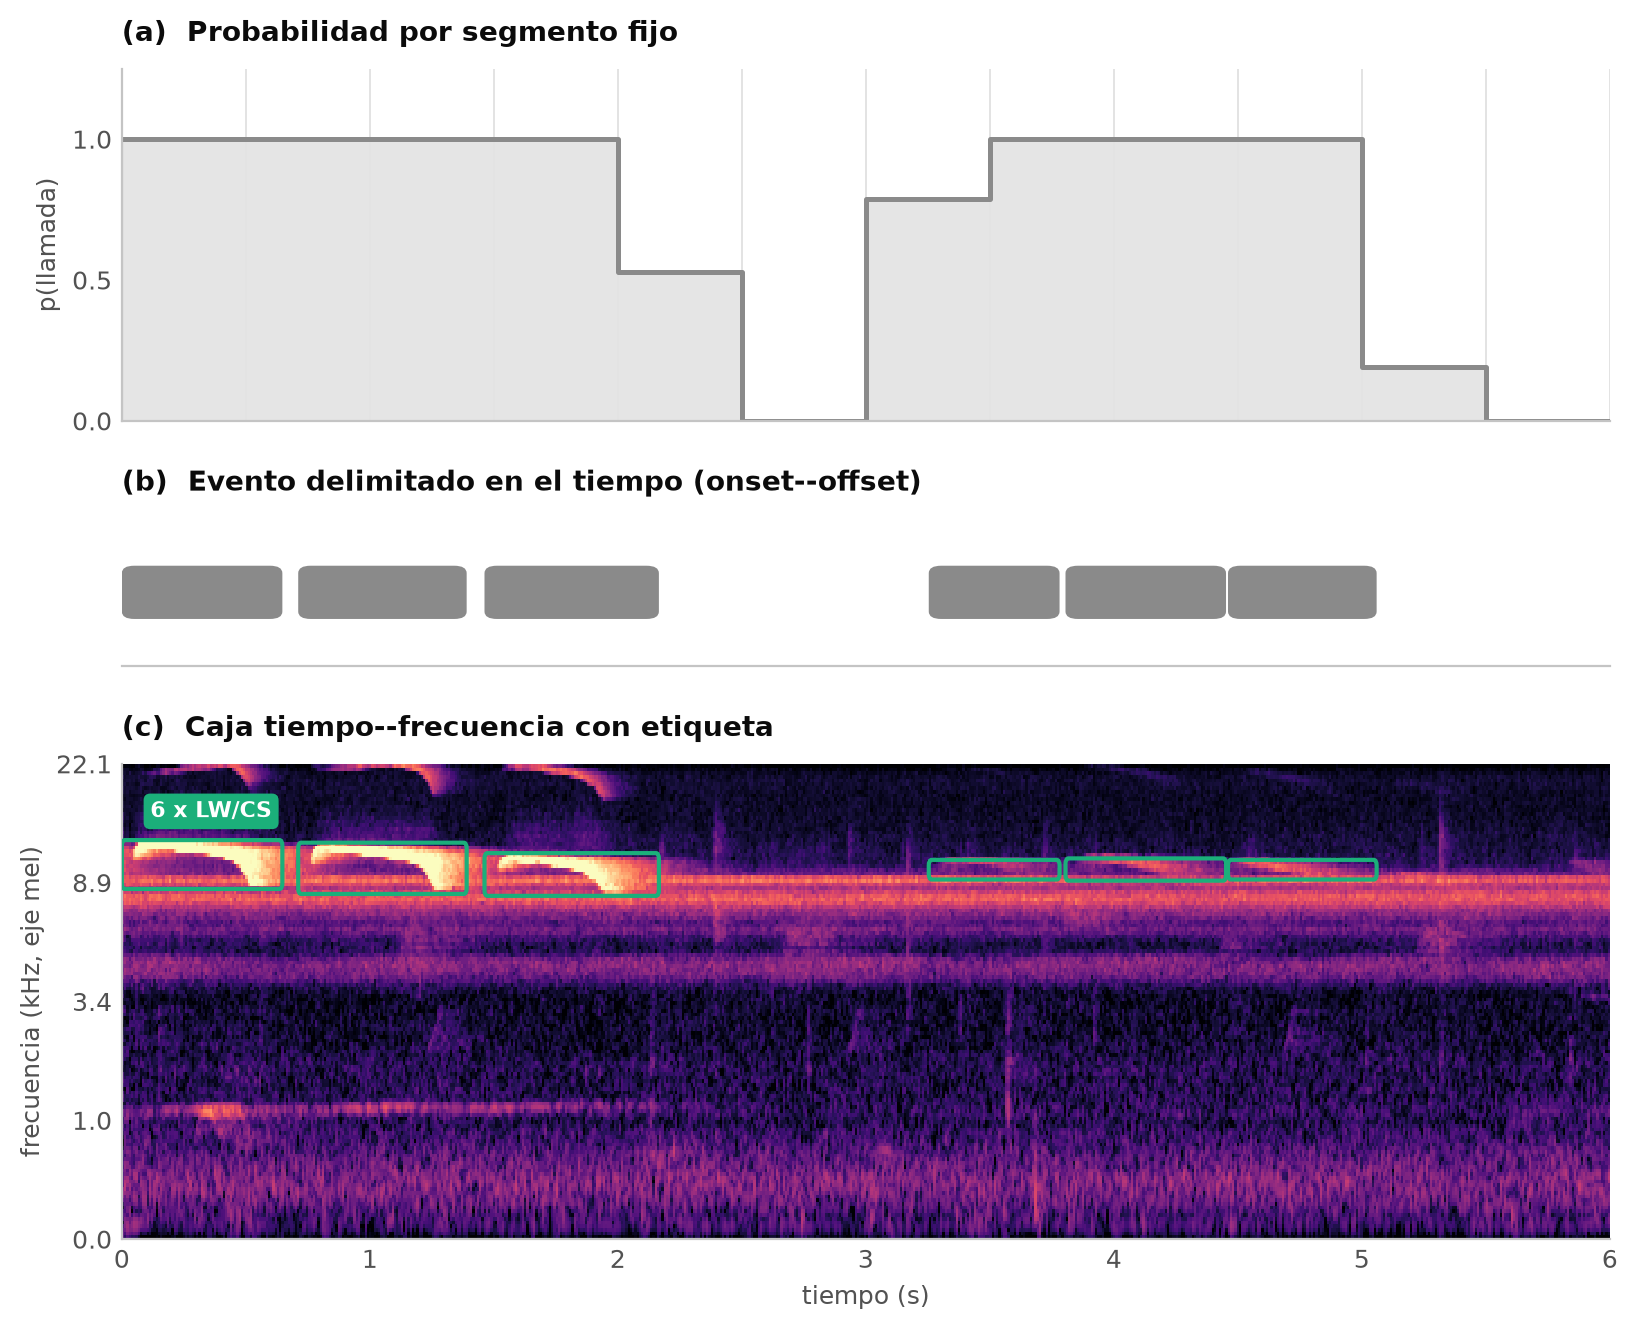
\includegraphics[width=\textwidth]{capitulos/01_generalidades/figures/output_forms.png}
\end{figure}

La forma (a) es la de los sistemas más difundidos. BirdNET identifica cientos de
especies de aves puntuando segmentos de 3\,s \citep{kahl_birdnet_2021}, y HOWLish
detecta aullidos de lobo sobre ejemplos de 0,96\,s cuyas predicciones promedia con
una ventana móvil \citep{Campos_Krofel_Rio-Maior_Renna_2025}. La forma (b)
delimita eventos, pero solo en el tiempo: los \textit{sound event bounding boxes}
formalizan cada predicción como una cuádrupla de clase, inicio, fin y confianza
\citep{ebbers_sound_2024}, y YOHO convierte la detección en una regresión de los
puntos de inicio y fin de cada clase \citep{venkatesh_you_2022}. En estas dos
formas se ubican los detectores construidos para primates: el sistema
semiautomático evaluado en el Parque Nacional Taï, en Costa de Marfil
\citep{heinicke_2015,kalan_towards_2015}, los reconocedores de aullidos de monos
aulladores en Brasil \citep{perez-granados_passive_2021,do_nascimento_passive_2021}
y la red que detecta las llamadas del langur de cabeza blanca en China
\citep{hong_deep_2026}. Su objetivo es establecer la presencia de una especie o de
su llamada característica, no anotar cada vocalización con su banda de frecuencia
y su tipo.

La forma (c) trata el espectrograma como una imagen y localiza cada vocalización
con los métodos de detección de objetos de la visión por computadora
\citep{pham_eventness_2018}.
Así se han detectado vocalizaciones de foca barbuda con YOLOv5
\citep{escobar-amado_computer_2024} y llamadas de aves migratorias nocturnas con
un detector de dos etapas, entrenado sobre anotaciones tiempo--frecuencia que
recolectaron decenas de aficionados \citep{airale_nbm_2025}. En primates, el
antecedente más cercano que se identificó es el uso de DeepSqueak, un programa de
detección de cajas desarrollado para roedores, sobre vocalizaciones del lémur
ratón gris grabadas en cautiverio, con una clasificación posterior del tipo de
llamada \citep{romero-mujalli_utilizing_2021}.

\subsection{Vacío}
\label{sec:vacio}

El vacío tiene dos ejes, y esta tesis se ubica en su cruce
(Tabla~\ref{tab:vacio}). Las filas de la tabla separan los taxones según los datos
anotados de que disponen; las columnas separan las dos clases de salida que
importan para la anotación: la que indica dónde hay una llamada, por segmento o
por intervalo temporal, y la que entrega la caja tiempo--frecuencia con su
etiqueta. Cada celda cita los trabajos que la ocupan.

\begin{table}[htbp]
    \centering
    \caption{Vacío de la investigación}
    \label{tab:vacio}
    \small
    \begin{tabular}{@{}L{3.6cm}L{5.1cm}L{5.1cm}@{}}
        \toprule
                                                       & \thead[l]{Presencia por segmento \\ o intervalo temporal}
                                                       & \thead[l]{Caja tiempo--frecuencia \\ con su etiqueta} \\
        \midrule
        \textbf{Aves y otros taxones con datos anotados} &
        BirdNET \citep{kahl_birdnet_2021}; lobos \citep{Campos_Krofel_Rio-Maior_Renna_2025};
        SEBB y YOHO \citep{ebbers_sound_2024,venkatesh_you_2022}           &
        Aves migratorias \citep{airale_nbm_2025};
        foca barbuda \citep{escobar-amado_computer_2024}                                                                     \\
        \addlinespace
        \textbf{Primates fuera del Neotrópico}         &
        Taï, Costa de Marfil \citep{heinicke_2015,kalan_towards_2015};
        langur de cabeza blanca \citep{hong_deep_2026}                     &
        Lémur ratón gris, en cautiverio \citep{romero-mujalli_utilizing_2021}                                                \\
        \addlinespace
        \textbf{Primates neotropicales}                &
        Monos aulladores \citep{perez-granados_passive_2021,do_nascimento_passive_2021} &
        \textbf{Vacío: esta tesis}                                                                                           \\
        \bottomrule
    \end{tabular}
\end{table}

La tabla deja una sola celda sin trabajos: la de los primates neotropicales con
salida tiempo--frecuencia. Los antecedentes en primates neotropicales detectan la
presencia de una llamada, y los trabajos que entregan cajas lo hacen para otros
taxones o para primates grabados en cautiverio.

\rotulo{Eje del taxón.} La causa C1 ya documentó que para primates neotropicales
no existe un conjunto público con anotaciones tiempo--frecuencia
(Tabla~\ref{tab:xenocanto}). El contraste con las aves muestra que el obstáculo
es el taxón y no la región.
% TODO Añadir una segunda búsqueda documentada (Dryad, Zenodo o Macaulay
% Library) con la misma disciplina de término y fecha. Dos fuentes
% convergentes son mucho más difíciles de refutar que una sola.

De la Reserva Amazónica de Inkaterra, en Madre de Dios, la misma región de las
grabaciones de esta tesis, se publicó un conjunto de 21 grabaciones de una hora
de paisaje sonoro con 14\,798 cajas tiempo--frecuencia de 132 especies de aves
\citep{hopping_collection_2022}, y de dos localidades de Colombia, otro de
73,62 horas con 15\,372 anotaciones tiempo--frecuencia de 168 especies
\citep{ruiz_pteroset_2026}. Aun así, los autores de este último advierten que los
conjuntos con anotación temporal precisa siguen siendo escasos en los paisajes
sonoros tropicales \citep{ruiz_pteroset_2026}, y la investigación con PAM
terrestre se ha concentrado en murciélagos y en regiones templadas del hemisferio
norte \citep{sugai_terrestrial_2019}. Si las aves de la Amazonía apenas cuentan con
datos de este tipo, los primates no cuentan con ninguno.

\rotulo{Eje de la tarea.} El vacío tampoco es solo de datos. La salida que
necesita el especialista combina dos tareas que la literatura considera poco
exploradas: la detección de cajas tiempo--frecuencia, un área en gran medida
inexplorada pese a su utilidad para el analista \citep{zhu_sound_2025}, y la
clasificación fina del tipo de llamada, que en bioacústica se reconoce como un
desafío abierto antes que como una capacidad demostrada
\citep{nolasco_learning_2023}. A ellas se suma una tercera carencia. El ahorro
que aporta la asistencia se ha medido para detectar una o pocas especies
(sección~\ref{sec:magnitud}), pero ninguno de los trabajos revisados lo mide para
la anotación completa, con caja, especie y tipo de llamada: los que entregan cajas
tiempo--frecuencia reportan solo métricas del modelo
\citep{escobar-amado_computer_2024,airale_nbm_2025,zhu_sound_2025}.

\subsection{Alcance de la tesis}
\label{sec:alcance-tesis}

Esta tesis se ubica en el cruce de ambos ejes: responde a las dos causas del
árbol y mide su efecto sobre el problema central. La propuesta de solución es un sistema de
pre-anotación asistida, que el objetivo general define. Su alcance se limita a las ocho especies del
material entregado, a grabaciones ya recolectadas, sin trabajo de campo, y a la
pre-anotación: el especialista conserva la decisión final sobre cada caja. Así
delimitado, el proyecto abarca el ciclo
completo de un sistema de aprendizaje automático, desde la construcción de sus
datos hasta la medición de su efecto sobre el trabajo humano, y cada una de esas
etapas se formula a continuación como un objetivo.

% ===================================================================
\section{Objetivos}
\label{sec:objetivos}
% ===================================================================
% Los enunciados del OG y de los OE se copian literalmente de objetivos.md
% (texto congelado). Lo que cambió el 06-10-2026 es el texto que los explica:
% qué significa cada uno, a qué causa del árbol responde y cómo contribuye.

Los objetivos convierten el árbol de problemas en un plan de trabajo: el objetivo
general responde al problema central; OE1 y OE2, a una causa cada uno, y OE3
evalúa si el sistema reduce el problema central.

\subsection{Objetivo general}

\begin{quote}
    \textbf{OG.} Desarrollar y evaluar un sistema de pre-anotación asistida que
    proponga cajas tiempo--frecuencia con especie y tipo de llamada sobre
    grabaciones de PAM de primates amazónicos, con el fin de reducir el tiempo de
    revisión experta.
\end{quote}

El objetivo general ataca el problema central en la magnitud que lo define, el
tiempo de especialista. Un sistema de \emph{pre-anotación asistida} propone
anotaciones para que el especialista las acepte, las corrija o las descarte en su
propia herramienta, en lugar de dibujarlas desde cero. Las propuestas tienen la misma forma que la
anotación manual de la Figura~\ref{fig:annotation-example}, una caja
tiempo--frecuencia con especie y tipo de llamada, porque solo así pueden
sustituirla en lugar de complementarla (sección~\ref{sec:soluciones}). Los
primates amazónicos del enunciado son las ocho especies de la
sección~\ref{sec:problema}. Y el criterio de éxito no es el desempeño del modelo,
que es un medio, sino la reducción del tiempo de revisión experta, que es la
magnitud del problema.

El encuadre asistido cuenta con respaldo en la literatura. La inteligencia
artificial no reemplaza la experiencia: conforme estos sistemas se estandarizan,
asumen el papel de pares expertos con quienes se consulta y debate, sin desplazar
el rol del experto ni el del trabajo colaborativo
\citep{stowell_computational_2022}. Y tiene precedentes cuantificados, entre ellos
el del sistema semiautomático para primates de Taï, cuyos ahorros de tiempo se
revisaron en la sección~\ref{sec:magnitud}.

El enunciado fija además un compromiso de diseño: priorizar la cobertura, es
decir, que el sistema encuentre la mayor parte de las vocalizaciones, aunque eso
suponga proponer también falsos positivos. En un flujo asistido, perder una
vocalización cuesta más que descartar una propuesta errónea, porque el
especialista revisa la salida de todos modos, y un detector puede resultar útil
aun con una precisión muy baja: HOWLish resulta útil operando con una precisión
de 0,006 \citep{Campos_Krofel_Rio-Maior_Renna_2025}. La contrapartida es que la carga que genera ese sesgo debe medirse, y de eso se ocupa
OE3.

\subsection{Objetivos específicos}

Los tres objetivos específicos se encadenan. El conjunto de datos que produce OE1
es el material con que se entrena y se mide el detector de OE2, y el detector de
OE2 es el sistema cuyo efecto sobre el trabajo del especialista mide OE3.

\begin{description}
    \item[OE1.] Definir un protocolo de curación y estandarización, y aplicarlo
          sobre las anotaciones entregadas por el equipo de investigación para construir
          un conjunto de datos consistente de cajas tiempo--frecuencia etiquetadas por
          especie y tipo de llamada.

    \item[OE2.] Implementar y evaluar un detector que reciba un espectrograma y
          devuelva cajas tiempo--frecuencia con especie, tipo de llamada y confianza,
          comparándolo con una línea base establecida.

    \item[OE3.] Cuantificar la reducción del tiempo de revisión que aporta el
          sistema y caracterizar sus errores mediante revisión experta de una muestra
          de predicciones.
\end{description}

El objetivo general tiene dos verbos, desarrollar y evaluar, y los objetivos
específicos los reparten: OE1 y OE2 desarrollan el sistema, y cada uno responde a
una causa del árbol; OE3 lo evalúa. Su propósito se entiende desde ese vínculo.

\rotulo{OE1 frente a C1.} Un detector solo puede aprender y evaluarse contra
anotaciones que sigan un criterio único, y la anotación manual no lo garantiza
(causa C1). Un \emph{protocolo de curación y
    estandarización} es un conjunto documentado de reglas que corrige lo
corregible sin volver a anotar el audio: unifica la escritura de las etiquetas
sobre un vocabulario cerrado de pares de especie y tipo de llamada, descarta el
ruido y las cajas inválidas y deja registro de cada decisión. Lo que no puede
corregirse, como el desacuerdo de criterio entre anotadores o el desbalance entre
especies, lo separa y lo deja documentado, de modo que la segunda pasada del
especialista se limita a lo que ninguna regla puede decidir. Aplicarlo produce el
conjunto de datos sobre el que trabajan OE2 y OE3.

\rotulo{OE2 frente a C2.} El detector ataca la búsqueda que describe la causa C2:
en lugar de recorrer la grabación entera, el especialista revisa las propuestas
que el detector encuentra. Es el componente que convierte el espectrograma de una
grabación en propuestas de anotación con la forma que usa el
especialista: cajas tiempo--frecuencia con especie, tipo de llamada y una
\emph{confianza}, el valor entre 0 y 1 con que el modelo puntúa cada propuesta y
que permite ordenarlas o filtrarlas. Compararlo con una \emph{línea base
    establecida}, un detector de eficacia ya documentada en la literatura,
entrenado y medido sobre los mismos datos, es lo que permite saber si la
arquitectura propuesta aporta algo frente a lo que ya existe.

\rotulo{OE3 frente al objetivo general.} OE3 no responde a una causa: es el
\emph{evaluar} del objetivo general, y mide si el sistema reduce la magnitud que
define el problema, el tiempo de especialista.
Cronometra la revisión del mismo tipo de material con y sin las propuestas del
detector, el ahorro que la literatura ha medido para detectar una especie pero no
para la anotación completa (sección~\ref{sec:vacio}). Y vuelve sobre la causa C1:
someter una muestra de predicciones al juicio de un especialista, la misma
segunda pasada que C1 describe, distingue los errores genuinos de las
vocalizaciones que la referencia omitió, de modo que mide también la calidad de
las anotaciones. Es el objetivo que responde, con una
cifra, si el sistema cumple el objetivo general.

% ===================================================================
\section{Resultados esperados}
\label{sec:resultados}
% ===================================================================
% Las tres tablas de IOV se copian literalmente de objetivos.md (texto
% congelado). El 06-10-2026 se reescribió todo lo que las rodea: antes de cada
% tabla se definen los términos técnicos que aparecen en ella, y después se
% justifica cada resultado por su aporte concreto. Los cambios propuestos sobre
% las propias tablas (medios de verificación accesibles, detalles técnicos en
% los IOV, rutas que ya no existen) esperan la decisión del autor: ver
% REESTRUCTURACION.md.

Cada objetivo específico se compromete con resultados esperados (RE): productos
tangibles que existirán al terminar el proyecto y que pueden inspeccionarse. Para
cada uno, la tabla correspondiente fija el \emph{medio de verificación}, es decir,
dónde puede comprobarse que el producto existe, y el \emph{indicador
    objetivamente verificable} (IOV), la condición observable que debe cumplir
para darse por logrado. Los términos técnicos de cada tabla se definen en los
párrafos que la preceden, y después de cada tabla se explica qué aporta cada
resultado a su objetivo. Los capítulos~\ref{cap:curacion}, \ref{cap:deteccion}
y~\ref{cap:utilidad} desarrollan un objetivo cada uno y verifican sus resultados
contra estas tablas.

\subsection{OE1: Protocolo y conjunto de datos curado}

OE1 parte de la causa C1: las anotaciones que entregó el equipo de investigación
son las únicas que existen para estas especies, pero no pueden usarse tal como
llegan para entrenar ni para evaluar un detector. La tesis no vuelve a anotar el
audio. Transforma ese material en un conjunto utilizable y se compromete con
tres productos, que la Tabla~\ref{tab:iov-oe1} detalla: las reglas de esa
transformación (RE1.1), el conjunto que resulta de aplicarlas (RE1.2) y el
documento que lo describe (RE1.3). Las grabaciones y las anotaciones originales
siguen siendo del equipo; la contribución de la tesis es esa capa derivada.

Cada regla del protocolo (RE1.1) responde a un defecto concreto del material
recibido, y el indicador las nombra por ese defecto. La \emph{normalización}
unifica los nombres de las columnas y la escritura de las etiquetas, y el
\emph{mapa de sinónimos} reúne en una sola clase las distintas grafías con que se
escribió. Las filas de \emph{ruido}, que marcan sonido de fondo en lugar de una
vocalización, y las \emph{cajas degeneradas}, con duración o ancho de banda
nulos, se descartan. Los
\emph{pares imposibles}, combinaciones de especie y tipo de llamada que no
existen en el repertorio de la especie, se corrigen. El recorte al \emph{límite
de Nyquist}, la frecuencia más alta que una grabación puede representar (la mitad
de su frecuencia de muestreo: 22,05\,kHz a 44,1\,kHz), elimina la parte de una
caja que excede lo grabado. Y los \emph{registros fuera de vocabulario}, cajas
cuya etiqueta no corresponde a ninguna clase admitida, se marcan para revisión en
lugar de descartarse.

El conjunto (RE1.2) se entrega \emph{particionado}, es decir, dividido en tres
subconjuntos sin elementos comunes: el de entrenamiento, con el que el modelo
ajusta sus parámetros; el de validación, con el que se eligen sus
configuraciones, y el de prueba, que se reserva para medir el desempeño final.
Las proporciones 60/22,5/17,5 indican el porcentaje del material que va a cada
uno. La división se hace por archivo de grabación porque el modelo no recibe
grabaciones enteras sino \emph{ventanas}, fragmentos de 3\,s tomados cada 1,5\,s
y por tanto solapados: dos ventanas vecinas de una misma grabación son casi
iguales, y repartirlas entre entrenamiento y prueba inflaría el resultado. Cada
ventana se guarda como un espectrograma log-mel, la representación del audio que
recibe el modelo (sección~\ref{sec:frontends}), en tres archivos \texttt{.pt},
uno por subconjunto, y el archivo \texttt{meta.json} registra los parámetros con
que se generaron. Por último, la \emph{ficha del conjunto} (RE1.3), conocida en
inglés como \textit{datasheet}, es el documento que describe la composición, el
origen, el proceso de construcción, los usos recomendados y las limitaciones de
un conjunto de datos \citep{gebru_2021}.

\begin{table}[htbp]
    \centering
    \caption{IOV de OE1}
    \label{tab:iov-oe1}
    \small
    \begin{tabular}{@{}L{1.0cm}L{3.7cm}L{3.2cm}L{6.1cm}@{}}
        \toprule
        \textbf{RE} & \textbf{Resultado} & \textbf{Medio de verificación} & \textbf{Indicador objetivamente verificable (IOV)} \\
        \midrule
        RE1.1 & Protocolo de curación y estandarización documentado. & Documento del protocolo. & Define la normalización de columnas y etiquetas, el mapa de sinónimos, el descarte de ruido y cajas degeneradas, la corrección de pares imposibles, el recorte al límite de Nyquist y el tratamiento de registros fuera de vocabulario. \\
        \addlinespace
        RE1.2 & Conjunto acústico curado y particionado para el experimento. & Directorio \texttt{data/processed/}: etiquetas, metadatos y tres archivos \texttt{.pt}. & Los archivos procesados cargan sin error; \texttt{meta.json} registra la semilla, el criterio de selección, las exclusiones, la etiqueta usada y la normalización; el código divide por archivo de grabación con proporciones 60/22,5/17,5 y no por ventanas aisladas. \\
        \addlinespace
        RE1.3 & Ficha del conjunto derivado. & Capítulo de curación, README y metadatos del conjunto. & Describe las ocho especies, el vocabulario, la composición, el desbalance, el diccionario de campos, el ventaneo de 3 s con salto de 1,5 s, la normalización log-mel, las exclusiones y las limitaciones conocidas. \\
        \bottomrule
    \end{tabular}
\end{table}

\rotulo{Aporte de RE1.1.} El protocolo hace explícita y repetible la
estandarización que exige la causa C1: al quedar escrito como un conjunto de
reglas, puede aplicarse de nuevo cada vez que el equipo entregue más anotaciones,
y cualquier tercero puede comprobar qué se hizo con cada fila.

\rotulo{Aporte de RE1.2.} El conjunto curado y particionado es el insumo directo
de OE2 y la referencia contra la que OE3 compara. Que la partición sea por
grabación hace que el desempeño se mida sobre grabaciones que el modelo no vio al
entrenar, que es la situación en que el equipo lo usará: sobre grabaciones
nuevas.

\rotulo{Aporte de RE1.3.} La ficha cumple dos funciones. Permite que el equipo de
investigación, o un tercero, use el conjunto sin depender del autor. Y declara sus
límites (el desbalance entre especies, los sesgos de lo que se anotó, las clases
que quedaron fuera), que son también los límites de lo que OE2 y OE3 pueden
afirmar.

\subsection{OE2: Detector y evaluación}

OE2 responde a la causa C2: construye el detector que encuentra las
vocalizaciones en lugar del especialista, y lo evalúa. Se compromete con cinco
productos que siguen el orden del trabajo: diseñar el detector (RE2.1), construir
el \textit{pipeline} que lo entrena y lo aplica (RE2.2), compararlo con las líneas
base (RE2.3), entregar el modelo final en el formato de Raven (RE2.4) y publicar
el código y el modelo (RE2.5). La Tabla~\ref{tab:iov-oe2} los detalla, con
términos que conviene definir. Un \emph{detector} es un modelo que recibe el espectrograma de una ventana y
devuelve un conjunto de cajas, cada una con su clase y su confianza. La
arquitectura propuesta, AST-Deformable-DETR (RE2.1), combina dos piezas que el
Capítulo~\ref{cap:marco} describe: un extractor de características preentrenado
con audio, el \textit{Audio Spectrogram Transformer} (AST), y una cabeza de
detección de la familia DETR (\textit{DEtection TRansformer}), que predice directamente un conjunto de cajas. Su
\emph{dimensión}, su número de \emph{consultas} y su número de \emph{niveles} son
sus hiperparámetros principales: el tamaño de su representación interna, el
máximo de cajas que puede proponer por ventana y el número de escalas con que
analiza el espectrograma. El \textit{pipeline} (RE2.2) es la secuencia de
programas que lleva de las anotaciones a un modelo entrenado, y de este a las
predicciones sobre una grabación nueva; un \textit{checkpoint} (RE2.4) es el
archivo que guarda los pesos de un modelo entrenado, y \texttt{labels.json}, la
lista de clases que esos pesos predicen.

Las métricas de RE2.3 comparan las predicciones con las anotaciones. Una
predicción cuenta como \emph{verdadero positivo} cuando su caja se superpone lo
suficiente con una caja anotada de la misma clase, y esa superposición se mide
con el IoU (\textit{intersection over union}): el área común de las dos cajas
dividida por el área que cubren entre ambas, que vale 1 si coinciden y 0 si no se
tocan. Sobre esos aciertos se calculan el \textit{recall}, la fracción de
vocalizaciones anotadas que el detector encuentra; la \emph{precisión}, la
fracción de sus predicciones que son correctas, y F1, que combina ambas. La
precisión media (AP) resume la relación entre precisión y \textit{recall} a lo
largo de todos los umbrales de confianza \citep{lin_2014}, y se reporta con dos
exigencias de superposición, IoU 0,25 y 0,5. La matriz de confusión cuenta, para
cada clase anotada, a qué clase la asignó el detector. Por último, una
\emph{tabla de selección} es el archivo de texto con que Raven guarda y abre
anotaciones, y es el formato en que el modelo final entrega sus predicciones
(RE2.4).

\begin{table}[htbp]
    \centering
    \caption{IOV de OE2}
    \label{tab:iov-oe2}
    \small
    \begin{tabular}{@{}L{1.0cm}L{3.7cm}L{3.2cm}L{6.1cm}@{}}
        \toprule
        \textbf{RE} & \textbf{Resultado} & \textbf{Medio de verificación} & \textbf{Indicador objetivamente verificable (IOV)} \\
        \midrule
        RE2.1 & Diseño experimental, arquitectura propuesta y línea base. & Documento de diseño y módulo de arquitecturas. & Especifica la arquitectura AST-Deformable-DETR implementada con todos sus hiperparámetros, y define antes de entrenar la comparación con las líneas base declaradas: configuraciones, partición, métricas y regla de selección. \\
        \addlinespace
        RE2.2 & Pipeline reproducible de entrenamiento, evaluación e inferencia. & Scripts de datos, entrenamiento, evaluación e inferencia; módulos de \texttt{src/pipelines/}; \texttt{pyproject.toml} y manual técnico. & El pipeline genera los splits procesados, entrena desde un conjunto de configuración, evalúa un checkpoint y ejecuta inferencia sobre un WAV; las dependencias y comandos de ejecución están declarados. \\
        \addlinespace
        RE2.3 & Informe comparativo de resultados. & Informe de experimentación y archivos de métricas. & Reporta, como mínimo, recall, precisión, F1, IoU medio, AP a IoU 0,25 y 0,5, recall por clase y matriz de confusión; separa detección, encuadre y clasificación y justifica la selección del modelo. \\
        \addlinespace
        RE2.4 & Modelo final cargable y demostración funcional. & Checkpoint \texttt{.pth}, \texttt{labels.json} y ejecución de \texttt{src/infer.py}. & El checkpoint se carga sin claves incompatibles y la inferencia sobre un WAV produce un archivo tabulado con las columnas de Raven, incluidas coordenadas tiempo--frecuencia, especie, tipo de llamada y puntuación. \\
        \addlinespace
        RE2.5 & Código y modelo disponibles en un repositorio. & Repositorio de control de versiones. & La URL del repositorio permite localizar el código de curación, entrenamiento, evaluación e inferencia, junto con las instrucciones de ejecución y los artefactos del modelo final que se hayan decidido publicar. \\
        \bottomrule
    \end{tabular}
\end{table}

\rotulo{Aporte de RE2.1.} El documento de diseño fija qué se compara y con qué
regla antes de entrenar, para que la comparación no pueda ajustarse a posteriori
al resultado. Parte de formular la anotación como detección de objetos sobre el
espectrograma, la tercera forma de salida de la Figura~\ref{fig:output-forms}, y
fija como referencia una línea base establecida sobre espectrogramas
\citep{gonzalez_yolo-based_2025}.

\rotulo{Aporte de RE2.2.} El \textit{pipeline} reproducible permite regenerar
cada cifra del informe a partir de los datos y del código, y es también lo que el
equipo de investigación necesita para aplicar el sistema a grabaciones nuevas sin
depender del autor.

\rotulo{Aporte de RE2.3.} El informe comparativo dice cuánto acierta el detector y
dónde falla, y separa tres ejes porque cada fallo le cuesta al especialista una
corrección distinta: una vocalización no detectada lo obliga a dibujar la caja
completa, una caja mal encuadrada solo a ajustarla y una etiqueta errónea solo a
cambiarla. Exigir un IoU bajo responde a la borrosidad de las fronteras señalada
en la causa C1, y priorizar el \textit{recall}, al compromiso de cobertura del
objetivo general.

\rotulo{Aporte de RE2.4.} El modelo final, capaz de escribir sus predicciones como
tabla de selección de Raven, es lo que convierte el detector en pre-anotación: el
especialista abre la tabla sobre la grabación, en su propia herramienta, y recibe
propuestas con los mismos campos que su anotación: tiempo, frecuencia, especie,
tipo de llamada y confianza.

\rotulo{Aporte de RE2.5.} El repositorio permite localizar el código y el modelo
final, que es la condición para que un tercero compruebe RE2.1 a RE2.4 y para que
el equipo siga usando el sistema cuando la tesis termine.

\subsection{OE3: Tiempo de revisión y análisis de errores}

OE3 mide el efecto del sistema sobre el problema central, el tiempo del
especialista, y sobre la calidad de la referencia (causa C1). Se compromete con
tres productos: la metodología de la medición, fijada antes de medir (RE3.1); la
medición del tiempo de revisión (RE3.2), y el análisis de los errores (RE3.3). La
Tabla~\ref{tab:iov-oe3} los detalla. El \emph{punto de operación} (RE3.1) es la
configuración con que se usa el detector: el umbral de confianza por debajo del
cual una propuesta no se muestra al revisor, que se elige en validación con la
regla de la sección~\ref{sec:metodos}, y la supresión de no máximos (NMS), que,
cuando varias propuestas se superponen por encima de un IoU de 0,3, conserva
solo la de mayor confianza. Las dos \emph{condiciones} de RE3.2 son la
manual, en la que el especialista anota desde cero, y la asistida, en la que
revisa las propuestas del detector; el tiempo de cada una se expresa en minutos
por hora de audio, para que materiales de distinta duración sean comparables, y
el \emph{orden de revisión} se declara porque quien ya revisó un material lo
anota más rápido la segunda vez. En RE3.3, las predicciones \emph{de alta
    confianza} son las que superan con holgura el punto de operación, y sus errores
se clasifican en tres categorías: \emph{evento no anotado}, una vocalización real
que la anotación de referencia omitió; \emph{ruido}, una predicción sobre un
sonido que no es una vocalización de las especies estudiadas, y \emph{error de
    encuadre}, una vocalización correctamente detectada cuya caja no se ajusta a la
anotada.

\begin{table}[htbp]
    \centering
    \caption{IOV de OE3}
    \label{tab:iov-oe3}
    \small
    \begin{tabular}{@{}L{1.0cm}L{3.7cm}L{3.2cm}L{6.1cm}@{}}
        \toprule
        \textbf{RE} & \textbf{Resultado} & \textbf{Medio de verificación} & \textbf{Indicador objetivamente verificable (IOV)} \\
        \midrule
        RE3.1 & Metodología de validación comparativa. & Documento de metodología y protocolo de revisión experta. & Especifica el subconjunto de prueba, el punto de operación elegido en validación y el umbral de IoU para verdadero positivo, fijados antes de medir, las métricas, el emparejamiento y el procedimiento para revisar discrepancias y eventos potencialmente omitidos. \\
        \addlinespace
        RE3.2 & Medición comparativa del tiempo de revisión. & Informe de validación, registros de tiempo y medición de inferencia. & Reporta minutos por hora de audio en condición manual y asistida, describe el material comparable y el orden de revisión, y presenta el tiempo de procesamiento del modelo por hora de audio. No fija un porcentaje de ahorro antes de medirlo. \\
        \addlinespace
        RE3.3 & Análisis cualitativo de errores y hallazgos. & Informe de análisis y espectrogramas anotados. & Clasifica una muestra de predicciones de alta confianza en evento no anotado, ruido y error de encuadre, e incluye ejemplos visuales de aciertos, errores comunes y detecciones correctas ausentes de la anotación de referencia. \\
        \bottomrule
    \end{tabular}
\end{table}

De los tres resultados, RE3.2 es el que responde por el objetivo general; los
otros dos lo hacen interpretable. RE3.1 impide ajustar la medición al resultado,
y RE3.3 dice de qué están hechos los errores que el especialista corrige.

\rotulo{Aporte de RE3.1.} La metodología, redactada y fechada antes de ejecutar la
evaluación, fija el material de prueba, el punto de operación, el umbral de
emparejamiento, las métricas y el protocolo con que el revisor resuelve las
discrepancias, siguiendo el marco de tubería para la identificación automatizada
de sonidos de \citet{gibb_2018}. Fijarla de antemano impide elegir a posteriori el
umbral o la métrica que mejor favorezcan al resultado ya obtenido.

\rotulo{Aporte de RE3.2.} La medición comparativa es el resultado que responde al
objetivo general. Compara minutos por hora de audio en ambas condiciones, sobre
material comparable y con el orden de revisión declarado, y suma a la condición
asistida el tiempo de procesamiento del modelo, que también forma parte de su
costo. El indicador no fija de antemano un porcentaje de ahorro: se mide y se
reporta con sus condiciones, y los ahorros revisados en la
sección~\ref{sec:magnitud} son su punto de comparación. La medición se acompaña de
magnitudes que se derivan de la propia salida del sistema, como las propuestas
por hora de audio y la fracción de audio sin ninguna propuesta, que explican de
dónde sale el ahorro, al modo de la reducción de 22 veces del volumen que un
operador debía procesar en HOWLish \citep{Campos_Krofel_Rio-Maior_Renna_2025}.

\rotulo{Aporte de RE3.3.} El análisis de errores resuelve la dificultad que señala
la causa C1: saber cuánto del error aparente es del modelo y cuánto de una
referencia incompleta. La clasificación se apoya en la relación geométrica entre
la caja predicha y las cajas anotadas, que resume la Tabla~\ref{tab:taxonomia-fp}.

\begin{table}[htbp]
    \centering
    \caption{Taxonomía de discrepancias}
    \label{tab:taxonomia-fp}
    \small
    \begin{tabular}{@{}L{1.0cm}L{2.5cm}L{5.2cm}L{1.8cm}L{3.1cm}@{}}
        \toprule
        \textbf{Tipo} & \textbf{Discrepancia} & \textbf{Definición} & \thead[l]{¿Sin\\experto?} & \thead[l]{Categoría\\en RE3.3} \\
        \midrule
        A & Encuadre  & Solapa con una anotación de la misma clase, pero con IoU inferior al umbral de emparejamiento.                       & Sí & Error de encuadre \\
        \addlinespace
        B & Unidad    & Varias predicciones sobre una misma anotación, o una predicción sobre varias anotaciones: división y fusión.          & Sí & Error de encuadre \\
        \addlinespace
        C & Clase     & Encuadre correcto sobre una anotación, con etiqueta de especie o de tipo de llamada incorrecta.                       & Sí & Error de clase, que se reporta aparte \\
        \addlinespace
        D & Región sin anotación & No solapa con ninguna caja anotada. Puede ser un evento omitido por la referencia o un falso positivo genuino. & \textbf{No} & Evento no anotado o ruido, según el revisor \\
        \bottomrule
    \end{tabular}
\end{table}

La última columna de la tabla indica a qué categoría de RE3.3 corresponde cada
tipo. Los tipos A y B quedan determinados por la geometría y son errores de
encuadre; el tipo C, una etiqueta equivocada sobre una caja correcta, no pertenece
a ninguna de las tres categorías comprometidas y se reporta aparte, y el tipo D,
las predicciones que no se superponen con ninguna anotación, es el que el revisor
experto resuelve entre evento no anotado y ruido. Los dos modos de error que
documenta \citet{zhu_sound_2025}, una caja anotada detectada como varias y varias
detectadas como una, corresponden al tipo B, y la borrosidad de las fronteras que
ese mismo trabajo describe es lo que hace necesario el tipo A.

\rotulo{Limitación declarada.} La resolución de las predicciones de alta
confianza situadas en regiones sin anotación (tipo D) entre eventos omitidos por
la referencia y falsos positivos genuinos depende del criterio experto, y este
trabajo lo obtiene sobre una muestra, no sobre el total. Lo que quede fuera de
esa muestra se caracteriza geométricamente y se reporta como una cantidad
acotada; el tamaño de la muestra y la disponibilidad del equipo de investigación
son, por tanto, una limitación del alcance de RE3.3, y como tal se declaran.

% ===================================================================
\section{Trazabilidad}
% ===================================================================

La Tabla~\ref{tab:trazabilidad} reúne la cadena que recorre este capítulo, del
problema a los productos comprometidos: cada causa del árbol se atiende con un
objetivo específico, OE3 mide el efecto sobre el problema central, cada objetivo
se concreta en sus resultados esperados y el objetivo general responde al
problema central. Los efectos E1 a E3 no se atacan
de forma directa: son lo que se espera aliviar si el objetivo general se cumple.
La tabla no reemplaza la justificación de cada vínculo, que está en las
secciones~\ref{sec:causas}, \ref{sec:objetivos} y~\ref{sec:resultados}; la
resume para que pueda leerse de un vistazo.

\begin{table}[htbp]
    \centering
    \caption{Trazabilidad del planteamiento}
    \label{tab:trazabilidad}
    \small
    \begin{tabular}{@{}L{4.1cm}L{1.8cm}L{2.3cm}L{5.6cm}@{}}
        \toprule
        \textbf{Elemento del árbol} & \textbf{Objetivo} & \textbf{Resultados} & \textbf{Aporte} \\
        \midrule
        C1: la anotación manual es inconsistente y exige una segunda pasada & OE1 & RE1.1 a RE1.3 & Conjunto curado, particionado y documentado \\
        \addlinespace
        C2: las vocalizaciones son escasas y breves, y encontrarlas a mano exige recorrer la grabación & OE2 & RE2.1 a RE2.5 & Detector que propone cajas con especie, tipo de llamada y confianza, en el formato de Raven \\
        \addlinespace
        Problema central (magnitud) y C1 (calidad de la referencia) & OE3 & RE3.1 a RE3.3 & Tiempo de revisión manual frente a asistido, y errores clasificados por un especialista \\
        \midrule
        Problema central                                     & OG  & Todos         & Sistema de pre-anotación asistida, evaluado por el tiempo de revisión experta \\
        \bottomrule
    \end{tabular}
\end{table}

Ninguna causa queda sin objetivo, y ningún objetivo queda sin un elemento del
árbol al que responder. Y aunque los once
resultados contribuyen al objetivo general, uno solo responde por él: RE3.2, la
medición del tiempo de revisión con y sin la asistencia del sistema.

% ===================================================================
\section{Métodos y procedimientos}
\label{sec:metodos}
% ===================================================================

\subsection{Metodología CRISP-DM}

El desarrollo se organiza siguiendo CRISP-DM (\textit{Cross-Industry Standard
    Process for Data Mining}), un marco iterativo, independiente de la industria y
de la herramienta, que proporciona una hoja de ruta general para proyectos de
minería de datos \citep{chapman_crisp-dm_2000}. Su estructura cíclica, desde la
comprensión del problema hasta el despliegue de la solución, se ajusta a un proyecto
de investigación aplicada en el que la comprensión de los datos, la
experimentación con modelos y la evaluación continua se realimentan entre sí.
La Figura~\ref{fig:crisp-dm} resume la correspondencia entre las seis fases, los
objetivos específicos y los capítulos de este documento.

\begin{figure}[tb]
    \centering
    \caption{CRISP-DM aplicado a este proyecto}
    \label{fig:crisp-dm}
    \begin{tikzpicture}[
            every node/.style={font=\footnotesize},
            fase/.style={caja, draw=azul!70, fill=azul!6, align=center,
                    text width=34mm, inner sep=4pt},
            ciclo/.style={-{Stealth[length=2mm]}, thick, draw=gris!90},
        ]
        \node[fase] (f1) at (0, 4.3)
        {\textbf{1. Comprensión de la investigación}\\[1pt]
            {\scriptsize Árbol de problemas, objetivos y criterios}\\[1pt]
            {\scriptsize\color{azul!80!black} Cap.~1}};
        \node[fase] (f2) at (4.6, 2.2)
        {\textbf{2. Comprensión de los datos}\\[1pt]
            {\scriptsize Exploración y calidad de las anotaciones}\\[1pt]
            {\scriptsize\color{azul!80!black} OE1 \sep Cap.~4}};
        \node[fase] (f3) at (4.6, -2.2)
        {\textbf{3. Preparación de datos}\\[1pt]
            {\scriptsize Curación, vocabulario, partición y ventaneo}\\[1pt]
            {\scriptsize\color{azul!80!black} OE1 \sep Cap.~4}};
        \node[fase] (f4) at (0, -4.3)
        {\textbf{4. Modelado}\\[1pt]
            {\scriptsize Detector de cajas y líneas base}\\[1pt]
            {\scriptsize\color{azul!80!black} OE2 \sep Cap.~5}};
        \node[fase] (f5) at (-4.6, -2.2)
        {\textbf{5. Evaluación}\\[1pt]
            {\scriptsize Métricas por eje, errores y tiempo de revisión}\\[1pt]
            {\scriptsize\color{azul!80!black} OE2, OE3 \sep Cap.~5, 6}};
        \node[fase] (f6) at (-4.6, 2.2)
        {\textbf{6. Despliegue}\\[1pt]
            {\scriptsize Inferencia por lotes y export a Raven}\\[1pt]
            {\scriptsize\color{azul!80!black} OE2 \sep Cap.~5}};
        \node[dato, align=center, text width=28mm] (datos) at (0, 0)
        {\textbf{DATOS}\\[1pt]{\scriptsize \nRecordingsRaw{} grabaciones\\
                \nKept{} anotaciones}};
        \foreach \a/\b in {f1/f2, f2/f3, f3/f4, f4/f5, f5/f6, f6/f1}
        \draw[ciclo] (\a) -- (\b);
    \end{tikzpicture}
\end{figure}

Las fases 2 y 3 corresponden a OE1; la 4 y la 6, a OE2, y la 5 se reparte entre
OE2 y OE3. Los párrafos siguientes describen cada fase.

\paragraph{Fase 1: Comprensión del negocio o de la investigación.}
Convierte el conocimiento del dominio y los objetivos del proyecto en una
definición formal del problema de minería de datos
\citep{chapman_crisp-dm_2000}. Esa traducción es el contenido de las secciones
anteriores de este capítulo: el problema se analiza con un árbol de problemas, y
de él derivan el objetivo general, los objetivos específicos y los resultados
esperados. Los criterios de éxito son a la vez técnicos, relacionados con el
desempeño en detección, encuadre y clasificación, y operativos, vinculados con el
tiempo de revisión experta que es la magnitud del problema, como recomienda el
marco para asegurar que el resultado sea útil y no solo correcto.

\paragraph{Fase 2: Comprensión de los datos.}
\label{sec:fase2}
Parte del material descrito en la sección~\ref{sec:dominio}: una carpeta por
especie con las grabaciones y, junto a cada una, la tabla de selección exportada
de Raven Pro, en la que cada fila registra las coordenadas de una caja, su
amplitud, su calidad y las etiquetas de especie y de tipo de llamada. La fase
comprende el análisis exploratorio (espectrogramas, distribución de clases,
duraciones y rangos de frecuencia) y la verificación de calidad: audios
corruptos, errores tipográficos y etiquetas inconsistentes.

\paragraph{Fase 3: Preparación de datos.}
\label{sec:fase3}
Comprende la limpieza y normalización de etiquetas sobre un vocabulario cerrado,
la selección de clases y la partición por grabación, el preprocesamiento del
audio, el cálculo de la representación tiempo--frecuencia y la segmentación de
las grabaciones largas en ventanas de duración fija con solapamiento. La
representación es el espectrograma log-mel, por la razón que da la
sección~\ref{sec:frontends}. El aumento de
datos se aplica al entrenar: variación de ganancia, mezcla con fondo del propio
entorno, corrimiento temporal y pegado de llamadas de otras ventanas, más una
perturbación leve de las cajas.

\paragraph{Fase 4: Modelado.}
\label{sec:fase4}
La forma de la salida no está en discusión: el sistema debe emitir la tupla
completa de la ecuación~\eqref{eq:tupla}, y esa exigencia excluye de antemano
toda arquitectura cuya cabeza produzca una probabilidad por trama o por segmento.
Lo que se compara, por tanto, no son familias de arquitectura sino
configuraciones que sí satisfacen la exigencia: la arquitectura propuesta sobre
un extractor de audio con cabeza de detección, y tres líneas base de detector
sobre espectrogramas: uno de dos etapas con propuestas de región, uno denso de
una etapa \citep{gonzalez_yolo-based_2025} y uno de conjuntos con extractor
preentrenado en imágenes.

La regla de decisión se fija antes de entrenar: gana la configuración con mayor
valor de la métrica principal definida en la Fase~5, medida sobre la partición de
\emph{validación}; la partición de prueba se reserva para reportar el desempeño
de la configuración ya elegida y no participa de la elección. La implementación
se realiza en PyTorch con código modular, separando la definición de la
arquitectura, el bucle de entrenamiento y las utilidades.

\paragraph{Fase 5: Evaluación.}
\label{sec:metricas}
Los modelos entrenados se evalúan sobre la partición de prueba y los resultados
se leen contra los criterios de éxito de la Fase~1. El análisis no se agota en
una cifra agregada: identifica qué clases se detectan mejor y peor, qué tipos de
error predominan, entre ellos la confusión entre especies acústicamente próximas,
los falsos positivos por ruido y los errores de localización en tiempo o en frecuencia, y
acompaña las cifras con ejemplos visualizados sobre el espectrograma.

Reportar varias métricas sin jerarquía permitiría elegir a posteriori la que
favorezca al modelo preferido. Para evitarlo, la Tabla~\ref{tab:metricas-sed}
asigna a cada una un rol fijado de antemano. Las métricas son las definidas al
presentar los resultados esperados de OE2 (sección~\ref{sec:resultados}).

\begin{table}[htbp]
    \centering
    \caption{Métricas de evaluación}
    \label{tab:metricas-sed}
    \small
    \begin{tabular}{@{}L{3.6cm}L{7.3cm}L{2.8cm}@{}}
        \toprule
        \textbf{Métrica}                                                 & \textbf{Definición} & \textbf{Rol} \\
        \midrule
        \textit{Recall} por evento, al punto de operación                &
        Proporción de eventos anotados recuperados por alguna predicción cuyo
        solapamiento con la caja anotada supera IoU 0,3, al umbral que la
        validación elige para ese modelo con precisión $\geq 0{,}70$. Se
        reporta con intervalo de confianza (IC).                              &
        \textbf{Principal}                                                                                    \\
        \addlinespace
        mAP a IoU 0,3                                                    &
        Precisión media sobre las clases de detección, integrando toda la curva
        precisión--\textit{recall}: no depende del umbral y por tanto no premia
        la calibración.                                                  &
        Secundaria y selección de \textit{checkpoint}                                                         \\
        \addlinespace
        FP/TP al punto de operación                                      &
        Falsos positivos por cada verdadero positivo: la carga de revisión que
        el experto asume por cada acierto.                               &
        Costo de revisión (OE3)                                                                               \\
        \addlinespace
        IoU mediano del encuadre                                         &
        Solapamiento entre la caja predicha y la anotada, sobre los eventos ya
        emparejados. Mide encuadre, no detección.                        &
        Encuadre                                                                                              \\
        \addlinespace
        AP a IoU 0,25 y a IoU 0,5                                        &
        La misma precisión media leída a un umbral de solapamiento laxo y a uno
        estricto: la distancia entre ambas mide cuánto se pierde al exigir
        encuadre.                                                        &
        Encuadre                                                                                              \\
        \addlinespace
        Acierto sobre pares emparejados                                  &
        Exactitud de la etiqueta de especie y tipo de llamada, condicionada a
        que la detección sea correcta.                                   &
        Clasificación                                                                                         \\
        \addlinespace
        Desempeño por clase                                              &
        \textit{Recall} individual para cada par de especie y tipo de llamada,
        con la causa atribuida a cada caída.                             &
        Diagnóstico                                                                                           \\
        \bottomrule
    \end{tabular}
\end{table}

La \textbf{métrica principal} es el \textit{recall} a nivel de evento, medido
al punto de operación que la partición de validación elige para cada
configuración: el umbral de confianza de mayor \textit{recall} entre los que
alcanzan una precisión de al menos 0,70. El \textit{recall} manda por el
compromiso de cobertura del objetivo general. Se acompaña siempre de su intervalo
de confianza por remuestreo de grabaciones, y dos configuraciones cuyos intervalos
se solapan se declaran no separadas por el experimento.

Un \textbf{umbral de confianza fijo y compartido} entre configuraciones no sirve
para esta comparación: la confianza que emite cada cabeza depende de su función
de pérdida y de cómo normaliza la puntuación, de modo que un mismo número cae en
puntos distintos de cada curva y mediría calibración tanto como detección. Por
eso cada modelo trae el suyo, elegido en validación, y viaja junto a su
\textit{checkpoint}.

El \textbf{criterio de selección de \textit{checkpoint}} dentro de una misma
corrida es la mAP a IoU 0,3 sobre validación: al no depender del umbral, elige la
época que mejor detecta y no la mejor calibrada. Es también la \textbf{métrica
    secundaria} de la comparación entre configuraciones, y la que decide cuando la
primaria no separa. El cociente \textbf{FP/TP al punto de operación} completa la
Tabla~\ref{tab:metricas-sed} porque es la magnitud que conecta esta fase con OE3.

\textbf{El acierto se decide a IoU 0,3 y el encuadre se puntúa aparte.}
Emparejar a 0,3 responde a si la llamada se \emph{encontró}, que es lo que decide
si el revisor la ve; exigir 0,5 en el mismo paso mezclaría esa pregunta con la de
si la caja quedó ajustada, cuando las fronteras del evento son borrosas incluso
entre anotadores \citep{zhu_sound_2025}. El encuadre se puntúa después, sobre los
pares ya emparejados, con el IoU mediano y con la AP a varios umbrales. La
Figura~\ref{fig:iou-criterion} muestra por qué conviene separar ambas preguntas:
compara tres predicciones con la anotación correspondiente, y junto al IoU da el
IoMin, la intersección dividida por el área de la caja menor.

\begin{figure}[htbp]
    \centering
    \caption{Criterio de IoU}
    \label{fig:iou-criterion}
    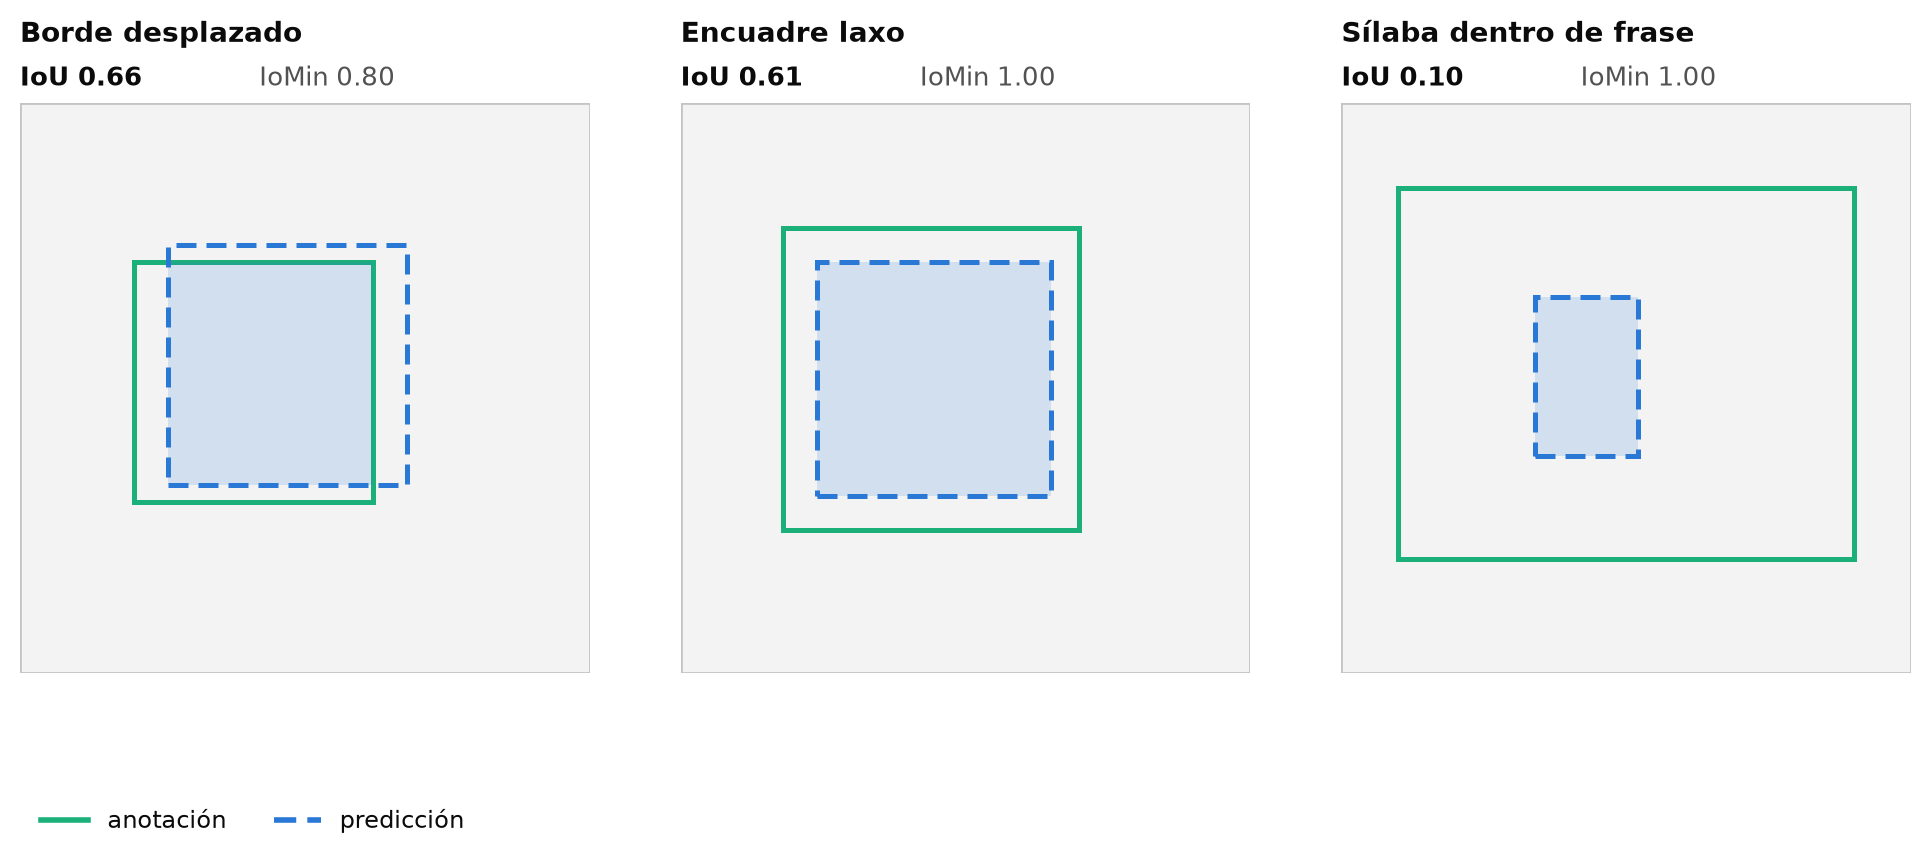
\includegraphics[width=\textwidth]{capitulos/01_generalidades/figures/iou_criterion.png}
\end{figure}

Los dos primeros casos, un borde desplazado y un encuadre laxo, superan los dos
umbrales aunque la caja predicha no coincida con la anotada. El tercero, una
sílaba predicha dentro de una frase anotada, queda muy por debajo de ambos aunque
la predicción esté íntegramente contenida en la anotación (IoMin 1,00): es el
anidamiento de unidades descrito en la causa C1, que ningún umbral de IoU resuelve
y que por eso se trata en la construcción del conjunto de datos.

El punto de operación con que OE3 cronometra la revisión asistida sale de esta
misma regla: es el umbral que la validación elige para el modelo seleccionado, y
queda fijado antes de medir el tiempo.

\paragraph{Fase 6: Despliegue.}
\label{sec:fase6}
En un proyecto de investigación el despliegue consiste en aplicar el modelo
final a un volumen de grabaciones que no participaron del entrenamiento ni de la
evaluación, y en producir con ellas tablas de anotación automáticas que el
analista pueda abrir directamente en Raven. El artefacto es un \textit{pipeline}
de inferencia que recibe un directorio de audio, aplica exactamente el mismo
preprocesamiento del entrenamiento, obtiene las predicciones crudas, ejecuta el
posprocesamiento y escribe la tabla de selección en el formato esperado.

\subsection{Herramientas}

Cada herramienta se justifica por el requisito que satisface y por la
alternativa que se descarta, no por sus virtudes generales; donde no hay
alternativa real, se dice. La Tabla~\ref{tab:herramientas} recoge las que
intervienen en el recorrido del dato, desde la lectura del audio hasta la tabla
que se abre en Raven.

\begin{table}[htbp]
    \centering
    \caption{Stack técnico: pipeline}
    \label{tab:herramientas}
    \small
    \begin{tabular}{@{}L{2.5cm}L{4.9cm}L{6.6cm}@{}}
        \toprule
        \textbf{Herramienta}                                                & \textbf{Función en el \textit{pipeline}} & \textbf{Por qué esta y no la alternativa} \\
        \midrule
        Python 3.12                                                         &
        Lenguaje de todo el sistema                                         &
        R y MATLAB carecen de implementaciones de referencia de detectores de
        objetos, que es el componente que no se va a reimplementar                                                                                                 \\
        \addlinespace
        Pandas                                                              &
        Consolidación, limpieza y particionado de las anotaciones tabulares &
        Procesar los archivos de Raven con scripts \textit{ad hoc} no deja
        registro reproducible de qué filas se descartaron y por qué                                                                                                \\
        \addlinespace
        NumPy                                                               &
        Representación en memoria del audio y de las cajas antes de pasar a
        tensores                                                            &
        Sin alternativa práctica: es la interfaz común entre SoundFile, PyTorch
        y Matplotlib                                                                                                                                               \\
        \addlinespace
        SoundFile y soxr                                                    &
        Lectura por bloques de las grabaciones y remuestreo a 44,1\,kHz     &
        Permiten leer solo la ventana pedida de un archivo de una hora, en lugar
        de cargarlo entero en memoria                                                                                                                              \\
        \addlinespace
        torchaudio                                                          &
        Cálculo del espectrograma mel que consume el modelo                 &
        Librosa devuelve arreglos de NumPy y obligaría a convertir en cada lote;
        aquí la transformada entrega tensores que van directamente al caché
        y al modelo                                                                                                                                               \\
        \addlinespace
        PyTorch                                                             &
        Definición, entrenamiento y evaluación del detector                 &
        Las implementaciones de referencia de detectores están mayoritariamente
        en PyTorch, y portarlas a otro marco no se justifica                                                                                                       \\
        \addlinespace
        Transformers                                                        &
        Carga del \textit{backbone} AST preentrenado en AudioSet            &
        Entrenar un transformador de espectrogramas desde cero excede los datos
        disponibles; la biblioteca aporta los pesos y la interpolación del
        \textit{embedding} posicional                                                                                                                              \\
        \addlinespace
        Raven Pro / Lite                                                    &
        Origen de las anotaciones y destino de las predicciones exportadas  &
        Sin alternativa: es la herramienta del analista, y su formato de tabla de
        selección es un requisito de RE2.4, no una elección de diseño                                                                                              \\
        \bottomrule
    \end{tabular}
\end{table}

De todas, solo Raven viene impuesta por el problema: su tabla de selección es el
formato en que el analista recibe las predicciones. Las demás responden sobre
todo a dos criterios: dejar registro reproducible (Pandas) y no hacer trabajo
redundante sobre el dato, es decir, leer solo la ventana pedida (SoundFile y
soxr), no convertir en cada lote (torchaudio) y reutilizar implementaciones y
pesos de referencia (PyTorch y Transformers). La
Tabla~\ref{tab:herramientas-dev} reúne lo que no toca el dato pero fija el
entorno y el estado del código con que se obtuvo cada resultado.

\begin{table}[htbp]
    \centering
    \caption{Stack técnico: desarrollo}
    \label{tab:herramientas-dev}
    \small
    \begin{tabular}{@{}L{2.5cm}L{4.9cm}L{6.6cm}@{}}
        \toprule
        \textbf{Herramienta}                                             & \textbf{Función} & \textbf{Por qué esta y no la alternativa} \\
        \midrule
        uv                                                               &
        Entorno virtual, resolución de dependencias y archivo de bloqueo &
        Instalar con \textit{pip} sin bloqueo deja libres las versiones
        transitivas, y sin ellas el entorno de una corrida antigua no se
        reconstruye igual                                                                                                               \\
        \addlinespace
        Matplotlib                                                       &
        Figuras del análisis exploratorio y de los resultados            &
        Sin alternativa que aporte algo distinto dentro del mismo ecosistema                                                            \\
        \addlinespace
        Ruff, ty y pytest                                                &
        Formato, análisis estático y pruebas del código                  &
        Las pruebas cubren la conversión entre sistemas de coordenadas de caja,
        donde un error silencioso desplazaría todas las métricas sin fallar                                                             \\
        \addlinespace
        Git                                                              &
        Versionado del código y de la configuración de cada experimento  &
        Sin alternativa: es la condición para asociar un resultado reportado a
        un estado exacto del código                                                                                                     \\
        \bottomrule
    \end{tabular}
\end{table}

El criterio común a ambas es la reproducibilidad: el conjunto de datos y cada
cifra del documento pueden regenerarse a partir del material primario, y la
subsección siguiente describe los procedimientos que lo garantizan.

\subsection{Procedimientos y reproducibilidad}
\label{sec:procedimientos}

Las fases anteriores describen qué se hace con los datos y por qué. Esta
subsección recoge únicamente lo operativo que no pertenece a ninguna fase en
particular porque atraviesa todas: cómo se custodia el material, cómo se
registran los experimentos y qué garantiza que un número reportado pueda volver a
obtenerse.

\rotulo{Custodia del material primario.} Los audios y sus anotaciones se
mantienen bajo una estructura de directorios fija que no se edita nunca a mano.
Toda transformación se produce por script a partir de ella y escribe en un
directorio derivado distinto. Esa separación es la que permite reconstruir el
conjunto de trabajo desde cero cada vez que el protocolo de curación cambia, y la
que impide que una corrección puntual quede sin registro.

\rotulo{Registro de experimentos.} Cada corrida queda asociada a un identificador
de configuración y a un \textit{commit} del repositorio. El bucle de
entrenamiento registra los hiperparámetros, guarda \textit{checkpoints} de forma
periódica y evalúa sobre validación a intervalos fijos. Los scripts de evaluación
son independientes de los de entrenamiento: cargan un \textit{checkpoint}
existente y recalculan las métricas, de modo que reproducir una cifra publicada
no exige reentrenar.

\rotulo{Respaldo y portabilidad.} El código y la configuración se sincronizan en
un repositorio remoto, y el entorno de ejecución se declara en un archivo de
dependencias versionado, para que la falla del equipo de desarrollo o la
ejecución en una máquina distinta no supongan rehacer trabajo. La gestión de la
bibliografía se centraliza en Zotero a lo largo de todo el proceso.

La planificación que ordena todo lo anterior en el tiempo, mediante la estructura de
desglose del trabajo, el cronograma, el presupuesto y la gestión de riesgos, se recoge
en el Anexo~\ref{anx:plan}, fuera del cuerpo, porque no aporta al argumento
científico y en el hilo del documento lo interrumpiría.

% ===================================================================
% CAPÍTULO 2
% ===================================================================
